\section{Tuần 6: Biến đổi Hình học, Làm trơn Ảnh và Phát hiện Biên cạnh}
\label{sec:week6}

Các câu hỏi trong tuần này dựa trên Bài giảng số 4 (\emph{3.2. Geometric Transformations})~\citep{xlav_lec4}, Bài giảng số 5 (\emph{3.3.1. Image Smoothing})~\citep{xlav_lec5} cùng phần bổ sung tiếng Việt \emph{Tuần 5: Làm trơn ảnh dựa trên miền không gian}~\citep{xlav_lec5b}, và Bài giảng số 6 (\emph{3.3.2. Edge Detection})~\citep{xlav_lec6}. Trong toàn bộ mục này, phép lọc được viết theo quy ước của bài giảng:
\begin{equation}
g(x, y) = \sum_{(i, j) \in O} f(x + i, y + j)\,h(i, j),
\label{eq:w6_filter}
\end{equation}
với $O$ là cửa sổ lân cận (mặt nạ) và $h$ là bộ lọc. Biểu thức này về mặt kỹ thuật là phép \emph{tương quan}; với $h$ đối xứng tâm ($h(i, j) = h(-i, -j)$) như mọi bộ lọc làm trơn và Laplace trong bài, nó trùng với phép tích chập $g = f * h$.

% =====================================================================
\subsection{Ví dụ về khó khăn khi thực hiện phép biến đổi hình học trên ảnh}
\label{subsec:w6_geo_difficulty}

\textit{Câu hỏi: Cho một ví dụ để thấy được những khó khăn khi thực hiện phép biến đổi hình học trên ảnh số.}

Trên mặt phẳng liên tục, một phép biến đổi hình học $(x', y') = \big(T_x(x, y), T_y(x, y)\big)$ (affine, song tuyến, đa thức~\citep{xlav_lec4}) chỉ đơn giản là di chuyển các điểm. Khó khăn xuất hiện vì ảnh số chỉ được định nghĩa trên \emph{lưới nguyên}: ảnh vào chỉ có giá trị tại các điểm nguyên, và ảnh ra cũng chỉ lưu được giá trị tại các điểm nguyên.

\textbf{Ví dụ 1: phóng to $2$ lần} ($x' = 2x$, $y' = 2y$, ví dụ trên bảng). Nếu duyệt ảnh vào và ``đẩy'' mỗi điểm sang vị trí mới (ánh xạ thuận), các điểm $(0, 0), (1, 0), (2, 0), \ldots$ đi tới $(0, 0), (2, 0), (4, 0), \ldots$. Các điểm ra có tọa độ lẻ như $(1, 0)$, $(3, 0)$, $(1, 1)$ \emph{không nhận được giá trị nào}: ảnh $2N \times 2M$ chỉ có $NM$ điểm được gán, tức $75\%$ điểm ảnh bị bỏ trống (lỗ). Ngược lại, khi thu nhỏ $2$ lần, bốn điểm vào cùng đổ về một điểm ra, phải quyết định giữ điểm nào (hay lấy trung bình), nếu không sẽ gây răng cưa (aliasing).

\textbf{Ví dụ 2: quay $30^\circ$ và phóng to $1{,}3$ lần.} Điểm $(10, 0)$ đi tới $\big(13\cos 30^\circ, 13\sin 30^\circ\big) = (11{,}26;\ 6{,}5)$ — tọa độ không nguyên. Làm tròn tọa độ rồi gán (ánh xạ thuận) dẫn tới hai lỗi đồng thời: nhiều ô của ảnh ra bị bỏ trống và một số ô bị gán hai lần. Hình~\ref{fig:w6_fwd_bwd} (cột 2) cho thấy $40{,}8\%$ điểm ảnh ra nằm trong vùng ảnh nhưng không nhận được giá trị nào (tô đỏ), tạo thành mẫu lỗ có tính chu kỳ, giống ví dụ chữ ``A'' bị xoay ở trang 5 của bài giảng.

\begin{figure}[ht]
\centering
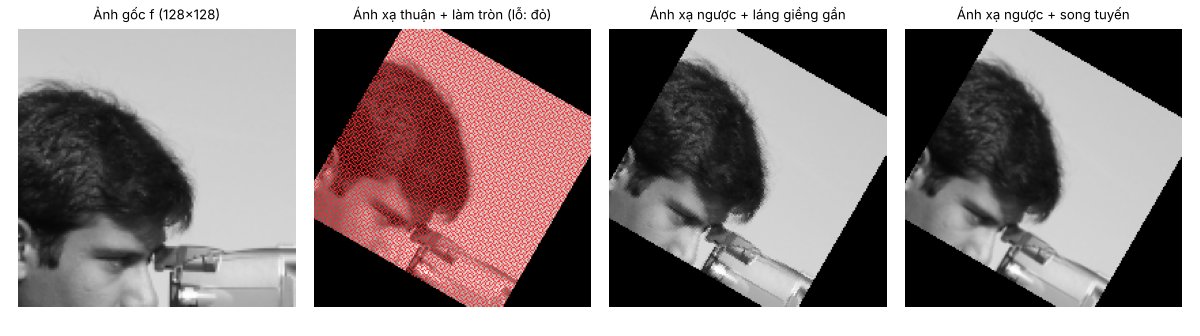
\includegraphics[width=\textwidth]{w6_forward_backward.png}
\caption{Quay $30^\circ$ và phóng to $1{,}3$ lần một vùng ảnh $128 \times 128$. Ánh xạ thuận để lại $40{,}8\%$ lỗ; ánh xạ ngược với nội suy láng giềng gần cho biên răng cưa; ánh xạ ngược với nội suy song tuyến cho kết quả trơn.}
\label{fig:w6_fwd_bwd}
\end{figure}

\textbf{Cách giải quyết và các khó khăn còn lại.}
\begin{enumerate}
    \item \emph{Ánh xạ ngược} (trang 8--9): duyệt từng điểm nguyên $(x', y')$ của ảnh ra, tính $(x, y) = T^{-1}(x', y')$ trên ảnh vào. Mọi điểm ra đều có giá trị, không còn lỗ. Khó khăn: cần $T^{-1}$ (với phép đa thức bậc cao thì $T^{-1}$ không có dạng tường minh, phải giải gần đúng).
    \item \emph{Nội suy độ sáng}: $(x, y)$ thường không nguyên, nên phải ước lượng $f(x, y)$ từ các điểm lân cận. Láng giềng gần nhất cho biên răng cưa (cột 3), nội suy song tuyến cho ảnh trơn nhưng hơi mờ (cột 4), nội suy bậc ba sắc nét hơn nhưng tốn tính toán hơn. Không phương pháp nội suy nào khôi phục được chi tiết đã mất.
    \item \emph{Biên ảnh}: $T^{-1}(x', y')$ có thể rơi ra ngoài ảnh vào (các góc đen trong Hình~\ref{fig:w6_fwd_bwd}); phải quy ước điền màu nền, lặp biên hay phản xạ.
    \item \emph{Thu nhỏ}: ánh xạ ngược chỉ lấy mẫu tại một điểm, nên khi thu nhỏ mạnh vẫn bị răng cưa; cần lọc thông thấp trước khi lấy mẫu.
    \item \emph{Biến đổi lặp lại}: mỗi lần nội suy đều làm mờ thêm và sai số tích lũy, nên khi cần ghép nhiều phép biến đổi phải nhân các ma trận trước rồi nội suy một lần.
\end{enumerate}

% =====================================================================
\subsection{Nhận xét về công thức nội suy tuyến tính (Bài giảng 4, trang 10)}
\label{subsec:w6_linear_interp_remark}

\textit{Câu hỏi: Trang 10 của Bài giảng 4 trình bày công thức nội suy tuyến tính độ sáng
\[
f'(x', y') = (1 - a)(1 - b)\,f(l, k) + a(1 - b)\,f(l + 1, k) + b(1 - a)\,f(l, k + 1) + ab\,f(l + 1, k + 1),
\]
với $l = \mathrm{round}(x)$, $a = x - l$, $k = \mathrm{round}(y)$, $b = y - k$, trong đó $(x, y) = T^{-1}(x', y')$~\citep{xlav_lec4}. Hãy nhận xét về biểu thức này.}

\textbf{1. Đây là nội suy \emph{song tuyến} (bilinear), ghép từ ba lần nội suy tuyến tính một chiều.} Như đã trình bày trên lớp, gọi $(x, k)$ và $(x, k + 1)$ là hai điểm trên cạnh dưới và cạnh trên của ô lưới chứa $(x, y)$. Nội suy theo phương $x$ trên hai cạnh rồi nội suy theo phương $y$:
\begin{align}
f(x, k) &= (1 - a) f(l, k) + a\,f(l + 1, k), \\
f(x, k + 1) &= (1 - a) f(l, k + 1) + a\,f(l + 1, k + 1), \\
f'(x', y') &= (1 - b) f(x, k) + b\,f(x, k + 1).
\end{align}
Thế hai đẳng thức đầu vào đẳng thức cuối ta được đúng công thức của bài giảng. Nội suy theo $y$ trước rồi theo $x$ cho cùng kết quả, vì công thức đối xứng theo hai phương.

\textbf{2. Định nghĩa $l = \mathrm{round}(x)$ cần sửa thành $l = \lfloor x \rfloor$.} Công thức chỉ là phép \emph{nội suy} khi $a, b \in [0, 1)$, tức $(l, k)$ là góc trên-trái của ô chứa $(x, y)$. Với $l = \mathrm{round}(x)$ thì $a \in [-0{,}5;\ 0{,}5)$ có thể âm. Ví dụ $x = 2{,}7$: $l = 3$, $a = -0{,}3$, công thức cho $1{,}3\,f(3, \cdot) - 0{,}3\,f(4, \cdot)$ — trọng số âm, dùng điểm $4$ nằm ngoài ô $[2, 3]$, tức là \emph{ngoại suy}. Giá trị đúng phải là $0{,}3\,f(2, \cdot) + 0{,}7\,f(3, \cdot)$. Vì vậy cần định nghĩa $l = \lfloor x \rfloor$, $k = \lfloor y \rfloor$ (hình vẽ trên bảng cũng ngầm dùng quy ước này: $(l, k)$ và $(l + 1, k + 1)$ là hai góc đối của ô chứa điểm). Ký hiệu $\mathrm{round}$ chỉ phù hợp với nội suy láng giềng gần nhất ở dòng trên của slide.

\textbf{3. Các trọng số là một tổ hợp lồi.} Bốn trọng số $(1 - a)(1 - b)$, $a(1 - b)$, $(1 - a)b$, $ab$ đều không âm và có tổng bằng $(1 - a + a)(1 - b + b) = 1$. Hệ quả: (i) vùng có độ sáng không đổi giữ nguyên độ sáng; (ii) giá trị nội suy luôn nằm giữa giá trị nhỏ nhất và lớn nhất của $4$ điểm lân cận, không có hiện tượng vượt quá (overshoot) như nội suy bậc ba; (iii) trọng số của mỗi góc bằng diện tích hình chữ nhật đối diện với góc đó, nên điểm càng gần góc nào thì góc đó càng có ảnh hưởng lớn.

\textbf{4. ``Tuyến tính'' theo từng biến, không tuyến tính theo cả hai.} Khai triển ra, $f'$ có dạng $c_0 + c_1 a + c_2 b + c_3 ab$: cố định $b$ thì tuyến tính theo $a$ và ngược lại, nhưng có số hạng $ab$. Mặt nội suy trên mỗi ô là một mặt yên ngựa (paraboloid hyperbolic), không phải mặt phẳng; dọc theo đường chéo của ô, giá trị thay đổi theo hàm bậc hai. Cùng dạng với phép biến đổi song tuyến $x' = a_0 + a_1 x + a_2 y + a_3 xy$ ở trang 7.

\textbf{5. Liên tục nhưng không trơn, và có tác dụng làm mờ.} Mặt nội suy liên tục qua các cạnh ô nhưng đạo hàm bị gãy tại các đường lưới. Nội suy song tuyến tương đương với việc lọc ảnh bằng một nhân tam giác, nên có tác dụng thông thấp nhẹ: biên bị làm mềm, không tạo ra chi tiết mới. So với láng giềng gần nhất (răng cưa, khối vuông) thì đẹp hơn rõ rệt (Hình~\ref{fig:w6_fwd_bwd}); so với nội suy bậc ba (bicubic, dùng $16$ điểm~\citep{keys1981cubic}) thì mờ hơn.

\textbf{6. Chi phí và biên ảnh.} Mỗi điểm cần $4$ lần đọc ảnh và khoảng $8$ phép nhân. Khi $l + 1$ hoặc $k + 1$ vượt ra ngoài ảnh (điểm nằm trên cạnh phải/dưới), phải kẹp chỉ số hoặc quy ước giá trị biên.

% =====================================================================
\subsection{So sánh thay đổi kích thước ảnh và siêu phân giải ảnh}
\label{subsec:w6_resize_vs_sr}

\textit{Câu hỏi: So sánh phép thay đổi kích thước ảnh (image resizing) bằng nội suy với kỹ thuật siêu phân giải ảnh (image super-resolution). Liệt kê các tiêu chí so sánh.}

Cả hai đều có thể biến ảnh $N \times M$ thành ảnh $sN \times sM$, nhưng khác nhau về bản chất: \emph{thay đổi kích thước} là bài toán \emph{lấy mẫu lại} một tín hiệu đã biết, còn \emph{siêu phân giải} là bài toán \emph{ngược}, ước lượng ảnh độ phân giải cao mà nếu bị làm mờ và lấy mẫu thưa sẽ cho ra ảnh quan sát được. Một ảnh độ phân giải thấp tương ứng với vô số ảnh độ phân giải cao, nên siêu phân giải cần thêm \emph{tri thức tiên nghiệm}: học từ dữ liệu~\citep{dong2016image,ledig2017photo}, hoặc kết hợp nhiều khung hình lệch nhau dưới mức điểm ảnh. Bảng~\ref{tab:w6_resize_sr} so sánh theo các tiêu chí.

\begin{table}[ht]
\centering
\scriptsize
\caption{So sánh thay đổi kích thước ảnh và siêu phân giải ảnh}
\label{tab:w6_resize_sr}
\renewcommand{\arraystretch}{1.3}
\begin{tabularx}{\textwidth}{|p{2.3cm}|X|X|}
\hline
\textbf{Tiêu chí} & \textbf{Thay đổi kích thước (nội suy)} & \textbf{Siêu phân giải (SR)} \\
\hline
Mục tiêu & Đổi số điểm ảnh để hiển thị, lưu trữ, đưa vào mô hình & Khôi phục ảnh độ phân giải cao, có thêm chi tiết thật \\
\hline
Chiều biến đổi & Phóng to và thu nhỏ & Chỉ phóng to (thường $\times 2$, $\times 3$, $\times 4$, $\times 8$) \\
\hline
Nguồn thông tin & Chỉ các điểm ảnh lân cận trong ảnh vào & Ảnh vào cùng tri thức tiên nghiệm học từ dữ liệu lớn, hoặc nhiều khung hình \\
\hline
Nguyên lý & Hàm nội suy cố định (láng giềng gần, song tuyến, bậc ba, Lanczos) & Bài toán ngược: học ánh xạ thấp $\to$ cao (SRCNN, ESRGAN, mô hình khuếch tán) hoặc tối ưu với ràng buộc tiên nghiệm \\
\hline
Chi tiết tần số cao & Không tạo thêm; ảnh phóng to bị mờ, răng cưa & Tái tạo (ước lượng) cạnh sắc, kết cấu \\
\hline
Tính xác định & Tất định, dễ giải thích, có công thức đóng & Phụ thuộc mô hình và dữ liệu huấn luyện; mô hình tạo sinh có thể ``bịa'' chi tiết không có thật \\
\hline
Hiện tượng lỗi & Mờ, răng cưa, viền chuông (bậc ba, Lanczos) & Ảo giác chi tiết, kết cấu giả, lỗi khi gặp ảnh khác miền huấn luyện \\
\hline
Đánh giá & Thường không cần đánh giá & PSNR, SSIM~\citep{wang2004image} (độ trung thực) và các độ đo cảm nhận như LPIPS, khảo sát người xem \\
\hline
Chi phí tính toán & Rất thấp, $O(1)$ mỗi điểm ảnh, thời gian thực trên CPU & Cao (hàng triệu tham số), thường cần GPU \\
\hline
Dữ liệu cần thiết & Không cần & Cần tập cặp ảnh thấp -- cao lớn \\
\hline
Ứng dụng & Hiển thị, tạo thumbnail, chuẩn hóa kích thước đầu vào mạng, tăng cường dữ liệu & Nâng cấp video cũ, ảnh vệ tinh, ảnh y khoa, camera giám sát, phóng to ảnh chụp \\
\hline
Độ tin cậy với dữ liệu nhạy cảm & Cao: không thêm thông tin & Phải thận trọng khi dùng làm bằng chứng (pháp y, chẩn đoán) vì chi tiết có thể là suy diễn \\
\hline
\end{tabularx}
\end{table}

Hai kỹ thuật cũng liên quan với nhau: nội suy bậc ba thường là \emph{điểm xuất phát} hoặc \emph{mức so sánh cơ sở} của SR (SRCNN phóng to bằng bicubic trước rồi mới học phần chi tiết~\citep{dong2016image}), còn bộ dữ liệu huấn luyện SR được tạo bằng cách \emph{thu nhỏ} ảnh thật.

% =====================================================================
\subsection{Dùng phép biến đổi hình học với nội suy tuyến tính để tăng cường dữ liệu}
\label{subsec:w6_augment_interp}

\textit{Câu hỏi: Sử dụng phép biến đổi (hình học) kết hợp nội suy tuyến tính để tăng cường dữ liệu (data augmentation).}

\textbf{Cách 1: biến đổi affine ngẫu nhiên kết hợp nội suy song tuyến.} Với mỗi ảnh huấn luyện, sinh một ma trận affine ngẫu nhiên gồm quay $\theta \sim \mathcal{U}(-20^\circ, 20^\circ)$, co giãn $s \sim \mathcal{U}(0{,}85;\ 1{,}15)$, trượt (shear) và tịnh tiến nhỏ quanh tâm ảnh, rồi tạo ảnh mới bằng ánh xạ ngược và nội suy song tuyến (Mục~\ref{subsec:w6_linear_interp_remark}). Giải thuật~\ref{alg:w6_augment} trình bày chi tiết.

\begin{algorithm}[ht]
\caption{Tăng cường dữ liệu bằng biến đổi affine ngẫu nhiên và nội suy song tuyến}
\label{alg:w6_augment}
\begin{algorithmic}[1]
\Require Ảnh $f$ kích thước $H \times W$ (xám hoặc màu); số ảnh cần sinh $K$
\Ensure $K$ ảnh tăng cường $g_1, \ldots, g_K$
\For{$t = 1, \ldots, K$}
    \State Sinh ngẫu nhiên $\theta, s, \text{sh}, (d_x, d_y)$; \quad $\mathbf{R} \gets s\begin{bmatrix}\cos\theta & -\sin\theta \\ \sin\theta & \cos\theta\end{bmatrix}\begin{bmatrix}1 & \text{sh} \\ 0 & 1\end{bmatrix}$
    \State $\mathbf{c} \gets (W/2, H/2)^T$; \quad $\mathbf{A} \gets \big[\mathbf{R} \mid \mathbf{c} - \mathbf{R}\mathbf{c} + (d_x, d_y)^T\big]$ \Comment{biến đổi quanh tâm ảnh}
    \State $\mathbf{M} \gets$ nghịch đảo của ma trận thuần nhất $3 \times 3$ $\begin{bmatrix}\mathbf{A} \\ 0\ 0\ 1\end{bmatrix}$
    \For{mỗi điểm $(x', y')$ của ảnh ra}
        \State $(x, y, 1)^T \gets \mathbf{M}\,(x', y', 1)^T$ \Comment{ánh xạ ngược}
        \If{$(x, y)$ nằm ngoài ảnh} \State $g_t(x', y') \gets 0$ \Comment{hoặc lặp biên, phản xạ}
        \Else
            \State $l \gets \lfloor x \rfloor$, $a \gets x - l$, $k \gets \lfloor y \rfloor$, $b \gets y - k$
            \State $g_t(x', y') \gets (1 - a)(1 - b)f(l, k) + a(1 - b)f(l + 1, k) + (1 - a)b\,f(l, k + 1) + ab\,f(l + 1, k + 1)$
        \EndIf
    \EndFor
\EndFor
\State \Return $g_1, \ldots, g_K$
\end{algorithmic}
\end{algorithm}

Với ảnh màu, công thức nội suy áp dụng độc lập cho từng kênh. Với bài toán phát hiện hoặc phân đoạn, các đỉnh hộp bao được biến đổi bằng chính $\mathbf{A}$, còn mặt nạ nhãn phải dùng nội suy láng giềng gần để không sinh ra nhãn trung gian vô nghĩa (ví dụ nhãn $1{,}5$ giữa lớp $1$ và lớp $2$).

\textbf{Cách 2: nội suy tuyến tính giữa hai mẫu (mixup).} Nội suy tuyến tính cũng có thể áp dụng \emph{giữa hai ảnh} thay vì giữa các điểm ảnh lân cận~\citep{zhang2018mixup}:
\begin{equation}
\tilde{x} = \lambda x_i + (1 - \lambda) x_j, \qquad \tilde{y} = \lambda y_i + (1 - \lambda) y_j, \qquad \lambda \sim \mathrm{Beta}(\alpha, \alpha),
\end{equation}
với $y$ là nhãn dạng one-hot. Mô hình được buộc phải dự đoán tuyến tính giữa các mẫu huấn luyện, giúp tăng khả năng tổng quát hóa và giảm hiện tượng quá tự tin. Mixup dùng chính tính chất tổ hợp lồi đã nêu ở Mục~\ref{subsec:w6_linear_interp_remark}, nhưng trong không gian các ảnh.

\textbf{Kết quả.} Hình~\ref{fig:w6_augment} (hàng trên) là $4$ ảnh sinh từ ảnh \texttt{astronaut} bằng Giải thuật~\ref{alg:w6_augment}, cài đặt trong tệp \texttt{XLAV/code/w6\_lib.py} (hàm \texttt{warp\_affine}, \texttt{random\_affine}); hàng dưới là mixup giữa \texttt{astronaut} và \texttt{chelsea} với các giá trị $\lambda$ khác nhau.

\begin{figure}[ht]
\centering
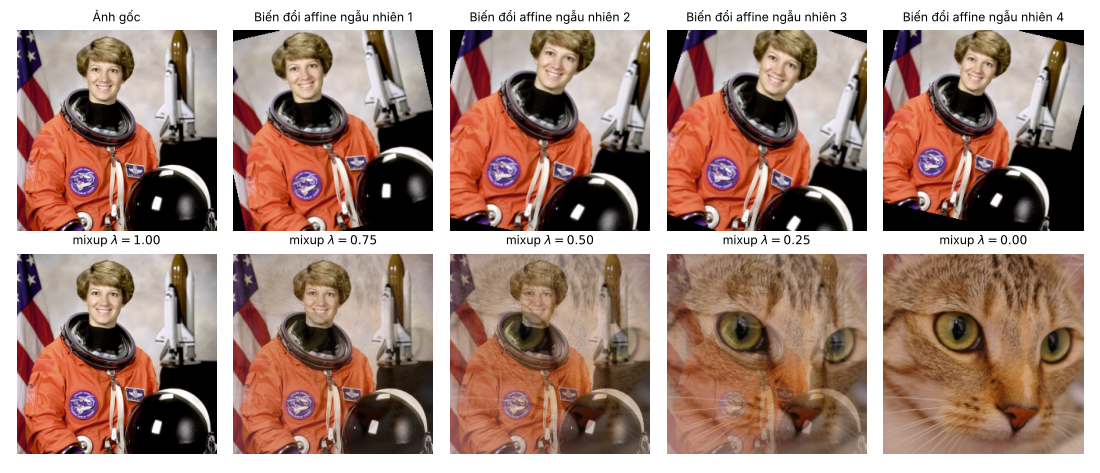
\includegraphics[width=\textwidth]{w6_augment.png}
\caption{Hàng trên: biến đổi affine ngẫu nhiên với nội suy song tuyến. Hàng dưới: mixup, nội suy tuyến tính giữa hai ảnh.}
\label{fig:w6_augment}
\end{figure}

% =====================================================================
\subsection{Hàm thêm nhiễu vào ảnh theo một hàm phân phối xác suất bất kỳ}
\label{subsec:w6_noise_func}

\textit{Câu hỏi: Dựa vào một hàm phân phối xác suất bất kỳ, viết hàm thêm nhiễu vào ảnh.}

\textbf{Cơ sở: phương pháp biến đổi ngược (inverse transform sampling).} Cho biến ngẫu nhiên $X$ có hàm phân phối tích lũy (CDF) $F(x) = P(X \le x) = \int_{-\infty}^{x} p(t)\,dt$. Nếu $U \sim \mathcal{U}(0, 1)$ thì $X' = F^{-1}(U)$ có cùng phân phối với $X$, vì
\begin{equation}
P(X' \le x) = P\big(F^{-1}(U) \le x\big) = P\big(U \le F(x)\big) = F(x),
\end{equation}
trong đó đẳng thức thứ hai dùng tính đơn điệu tăng của $F$ và đẳng thức cuối dùng $P(U \le u) = u$. Vì vậy chỉ cần một bộ sinh số ngẫu nhiên đều là sinh được nhiễu theo \emph{bất kỳ} hàm mật độ $p$ nào. Ý tưởng này giống với cân bằng lược đồ (Mục~\ref{subsec:w5_global}): $F$ biến một phân phối bất kỳ thành phân phối đều, còn $F^{-1}$ biến phân phối đều thành phân phối mong muốn.

\textbf{Cài đặt với hàm mật độ cho dưới dạng bảng.} Để hàm thêm nhiễu nhận được mọi phân phối (kể cả phân phối tự định nghĩa, không có công thức $F^{-1}$), ta nhận $p$ dưới dạng các giá trị trên một lưới điểm $z_0 < z_1 < \ldots < z_m$, tính CDF bằng tổng tích lũy, chuẩn hóa, và tính $F^{-1}(u)$ bằng nội suy tuyến tính trên bảng $(F(z_i), z_i)$. Hàm hỗ trợ ba mô hình nhiễu: cộng $g = f + n$ (nhiễu Gauss, đều, Laplace), nhân $g = f(1 + n)$ (nhiễu đốm, speckle) và xung (một tỉ lệ điểm ảnh bị thay bằng giá trị ngẫu nhiên, như nhiễu muối tiêu). Mã nguồn trong tệp \texttt{XLAV/code/w6\_lib.py}:
\begin{lstlisting}[language=Python]
import numpy as np

def sample_from_pdf(pdf, support, size, rng):
    """Draw samples from any 1-D pdf given on a grid `support`."""
    p = np.clip(np.asarray(pdf, float), 0, None)
    cdf = np.cumsum(p); cdf /= cdf[-1]          # F on the grid, F(z_m) = 1
    u = rng.random(size)                        # U ~ Uniform(0, 1)
    return np.interp(u, cdf, support)           # x = F^{-1}(u)

def add_noise(f, pdf, support, mode='additive', amount=1.0, rng=None):
    """additive: g = f + n;  multiplicative: g = f (1 + n);
       impulse: a fraction `amount` of the pixels is replaced by n ~ pdf."""
    rng = rng or np.random.default_rng()
    f = f.astype(np.float64)
    n = sample_from_pdf(pdf, support, f.shape, rng)
    if mode == 'additive':
        g = f + n
    elif mode == 'multiplicative':
        g = f * (1 + n)
    elif mode == 'impulse':
        g = np.where(rng.random(f.shape) < amount, n, f)
    return np.clip(np.round(g), 0, 255).astype(np.uint8)

# example: a user-defined bimodal pdf on [-100, 100]
z = np.linspace(-100, 100, 2001)
pdf = np.exp(-(z - 35) ** 2 / 50) + np.exp(-(z + 35) ** 2 / 50)
g = add_noise(f, pdf, z, rng=np.random.default_rng(0))
\end{lstlisting}

Hình~\ref{fig:w6_noise} minh họa với bốn phân phối: Gauss, đều, Laplace và một phân phối hai đỉnh tự định nghĩa. Lược đồ của $200.000$ mẫu sinh ra (màu xám) trùng khớp với hàm mật độ đã cho (đường đỏ), xác nhận tính đúng đắn của phương pháp. Lưu ý: bước cắt về $[0, 255]$ làm thay đổi phân phối thực của nhiễu ở vùng rất sáng hoặc rất tối; nếu cần nhiễu đúng phân phối cho mục đích đánh giá, nên lưu ảnh nhiễu dưới dạng số thực.

\begin{figure}[ht]
\centering
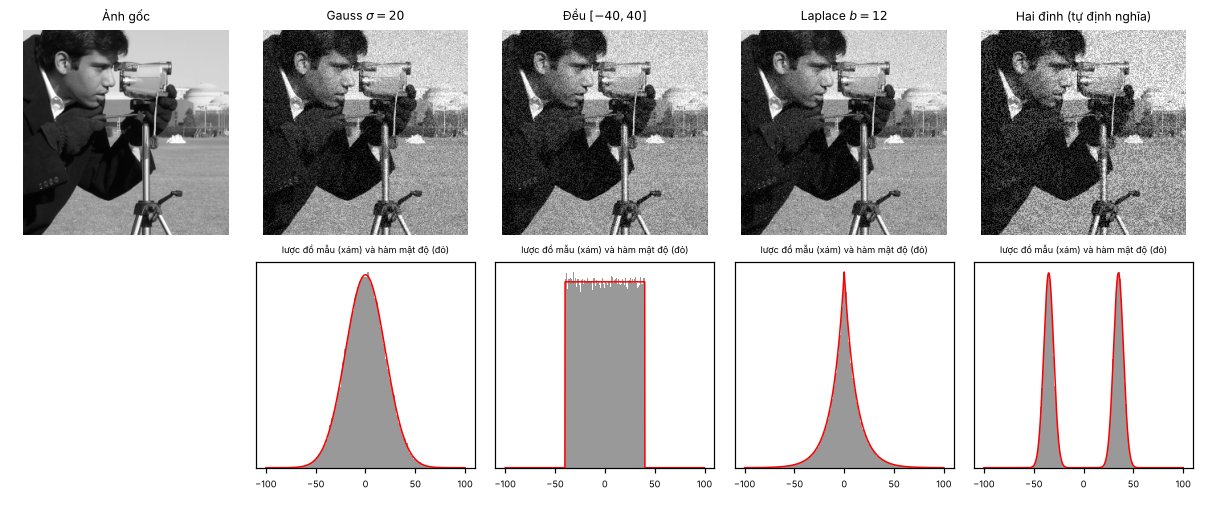
\includegraphics[width=\textwidth]{w6_noise.png}
\caption{Thêm nhiễu cộng theo bốn phân phối khác nhau bằng phương pháp biến đổi ngược. Hàng dưới: lược đồ mẫu nhiễu và hàm mật độ đã cho.}
\label{fig:w6_noise}
\end{figure}

% =====================================================================
\subsection{Vì sao phép tích chập có khả năng khử nhiễu}
\label{subsec:w6_conv_denoise}

\textit{Câu hỏi: Gọi $f$ là ảnh gốc, $n$ là nhiễu cộng và $g = f + n$ là ảnh quan sát. Lọc $g$ bằng bộ lọc $h$ ta có $g * h = f * h + n * h$. Hãy giải thích vì sao phép tích chập có khả năng khử nhiễu.}

Đẳng thức $g * h = f * h + n * h$ đến từ tính tuyến tính của tích chập: tín hiệu và nhiễu được lọc \emph{độc lập}. Phép lọc khử nhiễu được khi nó làm $n * h$ nhỏ đi rất nhiều trong khi $f * h$ gần như giữ nguyên $f$. Điều này đạt được nhờ hai tính chất khác nhau của tín hiệu và nhiễu.

\textbf{1. Nhiễu bị triệt tiêu khi lấy trung bình.} Giả sử nhiễu có kỳ vọng $0$, phương sai $\sigma^2$ và độc lập giữa các điểm ảnh. Với bộ lọc $h$ có $h(i, j) \ge 0$, $\sum h = 1$:
\begin{equation}
\mathbb{E}\big[(n * h)(x, y)\big] = \sum_{i, j} h(i, j)\,\mathbb{E}[n] = 0, \qquad
\mathrm{Var}\big[(n * h)(x, y)\big] = \sigma^2 \sum_{i, j} h(i, j)^2.
\end{equation}
Vì $\sum h = 1$ và có $K$ hệ số, theo bất đẳng thức Cauchy--Schwarz $\sum h^2 \ge \frac{1}{K}$, đẳng thức xảy ra khi $h$ là bộ lọc trung bình. Với bộ lọc trung bình $3 \times 3$: $\sum h^2 = 9 \cdot \frac{1}{81} = \frac{1}{9}$, độ lệch chuẩn của nhiễu giảm $3$ lần. Với bộ lọc Gauss $5 \times 5$, $\sigma_h = 1{,}1$ (Mục~\ref{subsec:w6_gauss_kernels}): $\sum h^2 \approx 0{,}071$, độ lệch chuẩn giảm khoảng $3{,}8$ lần. Nói cách khác, các giá trị nhiễu ngẫu nhiên lúc dương lúc âm nên \emph{bù trừ nhau} khi cộng có trọng số.

\textbf{2. Tín hiệu được bảo toàn vì ảnh trơn cục bộ.} Các điểm ảnh lân cận của ảnh tự nhiên có giá trị gần nhau (tương quan mạnh). Nếu $f$ là hằng số trong cửa sổ thì $f * h = f \sum h = f$; nếu $f$ là hàm tuyến tính trong cửa sổ và $h$ đối xứng thì $f * h = f$ (số hạng bậc nhất triệt tiêu). Vậy trong các vùng đồng nhất, tín hiệu đi qua bộ lọc gần như nguyên vẹn, còn nhiễu bị giảm $\sqrt{1/\sum h^2}$ lần.

\textbf{3. Góc nhìn tần số.} Theo định lý tích chập, $\mathcal{F}\{g * h\} = F \cdot H + N \cdot H$. Năng lượng của ảnh tự nhiên tập trung ở tần số thấp, còn nhiễu trắng trải đều trên mọi tần số. Bộ lọc làm trơn là bộ lọc thông thấp ($H \approx 1$ ở tần số thấp, $H \approx 0$ ở tần số cao): giữ gần hết năng lượng tín hiệu nhưng loại bỏ phần lớn năng lượng nhiễu, nên tỉ số tín hiệu trên nhiễu tăng.

\textbf{Thực nghiệm.} Với ảnh \texttt{camera} thêm nhiễu Gauss $\sigma = 20$, PSNR tăng từ $22{,}42$ dB lên $27{,}41$ dB (trung bình $3 \times 3$) và $27{,}80$ dB (Gauss $5 \times 5$) (Bảng~\ref{tab:w6_filters}).

\textbf{Giới hạn.} (i) Tại biên cạnh, $f$ không trơn nên $f * h \ne f$: biên bị nhòe — đây là cái giá phải trả. (ii) Lập luận trên cần nhiễu có kỳ vọng $0$ và phương sai hữu hạn, nhỏ so với tín hiệu. Với nhiễu xung (muối tiêu), một điểm sai lệch $\pm 255$ không bị triệt tiêu mà bị ``trải'' ra cả cửa sổ; khi đó bộ lọc phi tuyến như trung vị hiệu quả hơn nhiều (Mục~\ref{subsec:w6_filter_compare}).

% =====================================================================
\subsection{Hệ số của bộ lọc Gauss 2 chiều kích thước \texorpdfstring{$3$, $5$, $7$, $11$}{3, 5, 7, 11}}
\label{subsec:w6_gauss_kernels}

\textit{Câu hỏi: Xác định các hệ số của bộ lọc Gauss 2 chiều $h(i, j) = \frac{1}{2\pi\sigma^2}e^{-\frac{i^2 + j^2}{2\sigma^2}}$~\citep{xlav_lec5} với kích thước $3 \times 3$, $5 \times 5$, $7 \times 7$ và $11 \times 11$.}

\textbf{Chọn $\sigma$ theo kích thước.} Bộ lọc $n \times n$ ($n = 2r + 1$) chỉ có ý nghĩa khi $\sigma$ phù hợp với $r$: $\sigma$ quá lớn thì Gauss bị cắt cụt mạnh (gần với bộ lọc trung bình), $\sigma$ quá nhỏ thì các hệ số ở rìa gần bằng $0$, lãng phí. Ta dùng quy tắc của OpenCV
\begin{equation}
\sigma = 0{,}3\left(\frac{n - 1}{2} - 1\right) + 0{,}8,
\end{equation}
cho $\sigma = 0{,}8;\ 1{,}1;\ 1{,}4;\ 2{,}0$ tương ứng với $n = 3, 5, 7, 11$. (Một quy tắc khác là $r = \lceil 3\sigma \rceil$, tức cửa sổ phủ $\pm 3\sigma$ và chứa khoảng $99\%$ khối lượng của Gauss.)

\textbf{Chuẩn hóa.} Vì Gauss bị cắt cụt trong cửa sổ hữu hạn, tổng các hệ số tính theo công thức nhỏ hơn $1$, làm ảnh tối đi. Do đó sau khi lấy mẫu, ta chia cho tổng: $h(i, j) \leftarrow h(i, j) / \sum h$. Khi đó hằng số $\frac{1}{2\pi\sigma^2}$ không còn quan trọng.

\textbf{Tính tách được.} $e^{-\frac{i^2 + j^2}{2\sigma^2}} = e^{-\frac{i^2}{2\sigma^2}} \cdot e^{-\frac{j^2}{2\sigma^2}}$, nên $h = \mathbf{v}\mathbf{v}^T$ với $\mathbf{v}$ là Gauss 1 chiều đã chuẩn hóa. Lọc 2 chiều $n \times n$ có thể thay bằng hai lần lọc 1 chiều, giảm chi phí từ $n^2$ xuống $2n$ phép nhân mỗi điểm.

\textbf{Kết quả} (làm tròn $4$ chữ số; xấp xỉ nguyên thu được bằng cách chia cho hệ số nhỏ nhất rồi làm tròn):

$n = 3$, $\sigma = 0{,}8$, $\mathbf{v} = (0{,}2390;\ 0{,}5220;\ 0{,}2390)$:
\[
h_3 = \begin{bmatrix} 0{,}0571 & 0{,}1248 & 0{,}0571 \\ 0{,}1248 & 0{,}2725 & 0{,}1248 \\ 0{,}0571 & 0{,}1248 & 0{,}0571 \end{bmatrix}
\approx \frac{1}{17}\begin{bmatrix} 1 & 2 & 1 \\ 2 & 5 & 2 \\ 1 & 2 & 1 \end{bmatrix}.
\]

$n = 5$, $\sigma = 1{,}1$, $\mathbf{v} = (0{,}0708;\ 0{,}2445;\ 0{,}3695;\ 0{,}2445;\ 0{,}0708)$:
\[
h_5 = \begin{bmatrix}
0{,}0050 & 0{,}0173 & 0{,}0262 & 0{,}0173 & 0{,}0050 \\
0{,}0173 & 0{,}0598 & 0{,}0903 & 0{,}0598 & 0{,}0173 \\
0{,}0262 & 0{,}0903 & 0{,}1366 & 0{,}0903 & 0{,}0262 \\
0{,}0173 & 0{,}0598 & 0{,}0903 & 0{,}0598 & 0{,}0173 \\
0{,}0050 & 0{,}0173 & 0{,}0262 & 0{,}0173 & 0{,}0050
\end{bmatrix}
\approx \frac{1}{195}\begin{bmatrix}
1 & 3 & 5 & 3 & 1 \\ 3 & 12 & 18 & 12 & 3 \\ 5 & 18 & 27 & 18 & 5 \\ 3 & 12 & 18 & 12 & 3 \\ 1 & 3 & 5 & 3 & 1
\end{bmatrix}.
\]

$n = 7$, $\sigma = 1{,}4$, $\mathbf{v} = (0{,}0290;\ 0{,}1038;\ 0{,}2232;\ 0{,}2880;\ 0{,}2232;\ 0{,}1038;\ 0{,}0290)$:
\[
h_7 = \begin{bmatrix}
0{,}0008 & 0{,}0030 & 0{,}0065 & 0{,}0084 & 0{,}0065 & 0{,}0030 & 0{,}0008 \\
0{,}0030 & 0{,}0108 & 0{,}0232 & 0{,}0299 & 0{,}0232 & 0{,}0108 & 0{,}0030 \\
0{,}0065 & 0{,}0232 & 0{,}0498 & 0{,}0643 & 0{,}0498 & 0{,}0232 & 0{,}0065 \\
0{,}0084 & 0{,}0299 & 0{,}0643 & 0{,}0830 & 0{,}0643 & 0{,}0299 & 0{,}0084 \\
0{,}0065 & 0{,}0232 & 0{,}0498 & 0{,}0643 & 0{,}0498 & 0{,}0232 & 0{,}0065 \\
0{,}0030 & 0{,}0108 & 0{,}0232 & 0{,}0299 & 0{,}0232 & 0{,}0108 & 0{,}0030 \\
0{,}0008 & 0{,}0030 & 0{,}0065 & 0{,}0084 & 0{,}0065 & 0{,}0030 & 0{,}0008
\end{bmatrix},
\]
\[
h_7 \approx \frac{1}{1199}\begin{bmatrix}
1 & 4 & 8 & 10 & 8 & 4 & 1 \\
4 & 13 & 28 & 36 & 28 & 13 & 4 \\
8 & 28 & 59 & 76 & 59 & 28 & 8 \\
10 & 36 & 76 & 99 & 76 & 36 & 10 \\
8 & 28 & 59 & 76 & 59 & 28 & 8 \\
4 & 13 & 28 & 36 & 28 & 13 & 4 \\
1 & 4 & 8 & 10 & 8 & 4 & 1
\end{bmatrix}.
\]

$n = 11$, $\sigma = 2{,}0$. Ma trận $121$ hệ số được cho gọn dưới dạng tách được $h_{11} = \mathbf{v}\mathbf{v}^T$ với
\[
\mathbf{v} = (0{,}0088;\ 0{,}0271;\ 0{,}0651;\ 0{,}1216;\ 0{,}1770;\ 0{,}2006;\ 0{,}1770;\ 0{,}1216;\ 0{,}0651;\ 0{,}0271;\ 0{,}0088),
\]
tức $h_{11}(i, j) = v_i v_j$, ví dụ hệ số tâm $0{,}2006^2 = 0{,}0402$, hệ số góc $0{,}0088^2 \approx 0{,}0001$. Xấp xỉ nguyên: $\mathbf{v} \approx \frac{1}{113}(1, 3, 7, 14, 20, 23, 20, 14, 7, 3, 1)$, nên $h_{11} \approx \frac{1}{12769}\,\mathbf{u}\mathbf{u}^T$ với $\mathbf{u} = (1, 3, 7, 14, 20, 23, 20, 14, 7, 3, 1)$. Ở rìa cửa sổ $(r = 5 = 2{,}5\sigma)$ hệ số chỉ còn khoảng $4\%$ so với tâm theo mỗi phương.

Mã tính các hệ số là hàm \texttt{gaussian\_kernel(n, sigma)} trong \texttt{XLAV/code/w6\_lib.py}. Cùng một kích thước có thể có nhiều bộ hệ số khác nhau tùy cách chọn $\sigma$; khi so sánh với tài liệu khác cần ghi rõ $\sigma$.

% =====================================================================
\subsection{Chứng minh tính chất của bộ lọc trung vị (Bài giảng 5, trang 8)}
\label{subsec:w6_median_proof}

\textit{Câu hỏi: Trang 8 của Bài giảng 5 (\emph{Image smoothing}) nêu tính chất của bộ lọc trung vị $g(x, y) = \mathrm{med}\{f(x + i, y + j), (i, j) \in O\}$:
\[
\sum_{(i, j) \in O}\big|f(x + i, y + j) - \mathrm{med}\big| = \min_{(i', j') \in O}\ \sum_{(i, j) \in O}\big|f(x + i, y + j) - f(x + i', y + j')\big|,
\]
tức trung vị là giá trị trong cửa sổ có tổng khoảng cách tuyệt đối tới mọi giá trị khác là nhỏ nhất~\citep{xlav_lec5}. Hãy chứng minh tính chất này bằng cách thông thường hoặc bằng đạo hàm.}

\clarify{Câu hỏi ghi ``slide image smoothing trang 8''. Nhóm hiểu là trang 8 của Bài giảng 5 (tính chất trung vị). Trang 8 của phần bổ sung tiếng Việt (công thức phương sai của mặt nạ quay) được chứng minh ở Mục~\ref{subsec:w6_rotating_mask}. Cần xác nhận lại.}

Đặt $n = |O| = 2\nu + 1$ giá trị trong cửa sổ, sắp tăng dần $I_1 \le I_2 \le \ldots \le I_n$; khi đó $\mathrm{med} = I_{\nu + 1}$. Xét hàm
\begin{equation}
S(m) = \sum_{k=1}^{n} |I_k - m|, \qquad m \in \mathbb{R}.
\end{equation}
Ta chứng minh mạnh hơn: $I_{\nu + 1}$ cực tiểu $S$ trên \emph{toàn bộ} $\mathbb{R}$. Vì $I_{\nu + 1}$ cũng là một phần tử của cửa sổ, nó cực tiểu $S$ trên tập các giá trị trong cửa sổ, chính là đẳng thức cần chứng minh.

\textbf{Cách 1: dùng đạo hàm.} $S$ liên tục, tuyến tính từng đoạn và lồi (tổng các hàm lồi $|I_k - m|$). Với $m$ không trùng $I_k$ nào, $\frac{d}{dm}|I_k - m| = -1$ nếu $m < I_k$ và $+1$ nếu $m > I_k$, nên
\begin{equation}
S'(m) = \#\{k : I_k < m\} - \#\{k : I_k > m\}.
\end{equation}
\begin{itemize}
    \item Nếu $m < I_{\nu + 1}$: có ít nhất $\nu + 1$ phần tử ($I_{\nu + 1}, \ldots, I_n$) lớn hơn $m$ và nhiều nhất $\nu$ phần tử nhỏ hơn $m$, nên $S'(m) \le \nu - (\nu + 1) = -1 < 0$: $S$ giảm ngặt.
    \item Nếu $m > I_{\nu + 1}$: đối xứng, $S'(m) \ge (\nu + 1) - \nu = 1 > 0$: $S$ tăng ngặt.
\end{itemize}
$S$ liên tục, giảm trên $(-\infty, I_{\nu + 1}]$ và tăng trên $[I_{\nu + 1}, +\infty)$, nên đạt cực tiểu tại $m = I_{\nu + 1} = \mathrm{med}$. Theo ngôn ngữ đạo hàm dưới (subgradient), $0 \in \partial S(\mathrm{med})$ vì tại đó số phần tử bên trái bằng số phần tử bên phải.

\textbf{Cách 2: ghép cặp (không dùng đạo hàm).} Ghép các phần tử thành $\nu$ cặp đối xứng $(I_k, I_{n + 1 - k})$, $k = 1, \ldots, \nu$, và phần tử giữa $I_{\nu + 1}$. Theo bất đẳng thức tam giác, với mọi $m$:
\begin{equation}
|I_k - m| + |I_{n + 1 - k} - m| \ge I_{n + 1 - k} - I_k,
\end{equation}
dấu bằng xảy ra khi và chỉ khi $m \in [I_k, I_{n + 1 - k}]$. Ngoài ra $|I_{\nu + 1} - m| \ge 0$, dấu bằng khi $m = I_{\nu + 1}$. Cộng lại:
\begin{equation}
S(m) \ge \sum_{k=1}^{\nu}(I_{n + 1 - k} - I_k).
\end{equation}
Vế phải không phụ thuộc $m$. Các đoạn $[I_k, I_{n + 1 - k}]$ lồng nhau và cùng chứa $I_{\nu + 1}$, nên tại $m = I_{\nu + 1}$ mọi dấu bằng đều xảy ra: $S(\mathrm{med}) = \sum_{k=1}^{\nu}(I_{n + 1 - k} - I_k) \le S(m)$ với mọi $m$. \hfill $\square$

\textbf{Ý nghĩa.} Trung bình cộng là nghiệm của bài toán $\min_m \sum (I_k - m)^2$ (đạo hàm $2\sum(m - I_k) = 0 \Rightarrow m = \bar I$), còn trung vị là nghiệm của bài toán với chuẩn $L_1$. Sai số bình phương phạt rất nặng các giá trị ngoại lai, nên một điểm nhiễu $255$ kéo trung bình đi xa; sai số tuyệt đối chỉ phạt tuyến tính, và trung vị chỉ phụ thuộc vào \emph{thứ tự}, không phụ thuộc độ lớn của các giá trị ngoại lai. Ví dụ cửa sổ $\{10, 11, 12, 13, 255\}$: trung bình bằng $60{,}2$ còn trung vị bằng $12$. Đó là lý do bộ lọc trung vị khử nhiễu xung rất tốt và giữ được biên (trang 9).

% =====================================================================
\subsection{So sánh ba phương pháp lọc: trung bình, Gauss và trung vị}
\label{subsec:w6_filter_compare}

\textit{Câu hỏi: Lập bảng so sánh ba phương pháp lọc làm trơn trong bài giảng (lọc trung bình, lọc Gauss, lọc trung vị) theo các tiêu chí: khả năng khử nhiễu (tốt với loại nhiễu nào), phản ứng phụ trên biên cạnh, và các tiêu chí liên quan khác.}

Để có số liệu khách quan, nhóm thử nghiệm trên ảnh \texttt{camera} ($512 \times 512$) với hai loại nhiễu: nhiễu Gauss cộng $\sigma = 20$ và nhiễu muối tiêu $10\%$ ($5\%$ điểm thành $0$, $5\%$ thành $255$). Bảng~\ref{tab:w6_filters} cho PSNR (so với ảnh gốc, càng cao càng tốt) của từng bộ lọc. Để đo phản ứng trên biên, nhóm lọc một biên bậc lý tưởng $50 \to 200$ và đếm số điểm ảnh chuyển tiếp ở đầu ra. Bảng có thêm hai bộ lọc giữ biên ở các Mục~\ref{subsec:w6_gradient_weighted}, \ref{subsec:w6_rotating_mask} để so sánh. Kết quả trực quan với nhiễu muối tiêu ở Hình~\ref{fig:w6_smoothing}.

\begin{table}[ht]
\centering
\small
\caption{PSNR (dB) sau khi lọc ảnh \texttt{camera} và độ rộng vùng chuyển tiếp khi lọc một biên bậc}
\label{tab:w6_filters}
\renewcommand{\arraystretch}{1.2}
\begin{tabular}{|l|c|c|c|}
\hline
\textbf{Bộ lọc} & \textbf{Nhiễu Gauss $\sigma = 20$} & \textbf{Muối tiêu $10\%$} & \textbf{Biên bậc $50 \to 200$} \\
\hline
(ảnh nhiễu, chưa lọc) & $22{,}42$ & $14{,}79$ & -- \\
Trung bình $3 \times 3$ & $27{,}41$ & $22{,}48$ & $2$ điểm chuyển tiếp ($100$, $150$) \\
Gauss $5 \times 5$, $\sigma = 1{,}1$ & $\mathbf{27{,}80}$ & $23{,}51$ & $4$ điểm ($61$, $97$, $153$, $189$) \\
Trung vị $3 \times 3$ & $26{,}96$ & $\mathbf{29{,}59}$ & $0$ (giữ nguyên biên) \\
\hline
Trung bình trọng số gradient & $24{,}75$ & $17{,}77$ & $\approx 0$ \\
Mặt nạ quay & $26{,}71$ & $25{,}76$ & $0$ \\
\hline
\end{tabular}
\end{table}

\begin{figure}[ht]
\centering
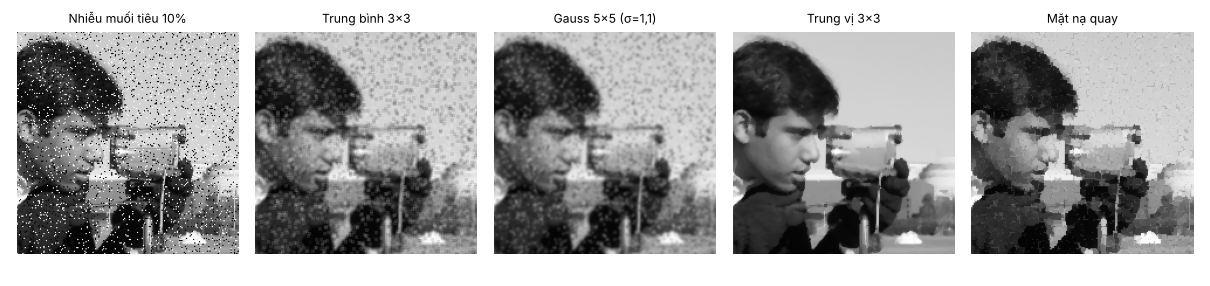
\includegraphics[width=\textwidth]{w6_smoothing.png}
\caption{Lọc nhiễu muối tiêu $10\%$ (vùng cắt của ảnh \texttt{camera}).}
\label{fig:w6_smoothing}
\end{figure}

\begin{table}[ht]
\centering
\scriptsize
\caption{So sánh ba phương pháp lọc làm trơn}
\label{tab:w6_three_filters}
\renewcommand{\arraystretch}{1.3}
\begin{tabularx}{\textwidth}{|p{2.2cm}|X|X|X|}
\hline
\textbf{Tiêu chí} & \textbf{Lọc trung bình} & \textbf{Lọc Gauss} & \textbf{Lọc trung vị} \\
\hline
Nguyên lý & Thay mỗi điểm bằng trung bình cộng các điểm trong cửa sổ, $h = \frac{1}{9}\mathbf{1}_{3 \times 3}$ & Trung bình có trọng số giảm dần theo khoảng cách, $h \propto e^{-(i^2 + j^2)/2\sigma^2}$ & Thay mỗi điểm bằng trung vị các điểm trong cửa sổ (thống kê thứ tự) \\
\hline
Loại bộ lọc & Tuyến tính, tích chập & Tuyến tính, tích chập, tách được & Phi tuyến, không phải tích chập \\
\hline
Tốt với loại nhiễu & Nhiễu cộng kỳ vọng $0$ (Gauss, đều); giảm phương sai tối đa với cùng kích thước (Mục~\ref{subsec:w6_conv_denoise}) & Nhiễu Gauss; tốt nhất trong thí nghiệm với nhiễu Gauss & Nhiễu xung (muối tiêu): hơn hai bộ lọc tuyến tính khoảng $6$--$7$ dB; với nhiễu Gauss kém hơn một chút \\
\hline
Kém với loại nhiễu & Nhiễu xung: điểm $0$/$255$ bị trải thành vết mờ & Nhiễu xung (như trung bình) & Nhiễu Gauss mật độ cao; nhiễu xung chiếm hơn nửa cửa sổ \\
\hline
Phản ứng phụ trên biên & Làm nhòe biên: biên bậc thành dốc rộng bằng cửa sổ; làm mất chi tiết nhỏ & Cũng nhòe nhưng mềm hơn, không có hiệu ứng khối; nhòe nhiều khi $\sigma$ lớn & Giữ nguyên biên bậc; nhưng xóa đường mảnh và điểm nhỏ hơn nửa cửa sổ, bo tròn góc nhọn \\
\hline
Đặc điểm phổ tần & Đáp ứng tần số dạng sinc, có thùy phụ, để lọt một số tần số cao & Đáp ứng cũng là Gauss, đơn điệu giảm, không có thùy phụ & Không định nghĩa được đáp ứng tần số \\
\hline
Độ phức tạp mỗi điểm & $O(1)$ với ảnh tích phân hoặc tổng trượt & $O(2n)$ nhờ tách được & $O(n^2 \log n)$ nếu sắp xếp; $O(n)$ với giải thuật lược đồ trượt \\
\hline
Tham số & Kích thước cửa sổ & Kích thước, $\sigma$ & Kích thước, hình dạng cửa sổ \\
\hline
\end{tabularx}
\end{table}

\textbf{Kết luận.} Với nhiễu Gauss, nên dùng bộ lọc Gauss (hoặc trung bình nếu cần nhanh). Với nhiễu xung, nên dùng bộ lọc trung vị. Khi cần giữ biên, cả ba đều có nhược điểm: hai bộ lọc tuyến tính làm nhòe biên, còn trung vị làm mất chi tiết mảnh. Điều này dẫn tới các bộ lọc giữ biên ở các mục sau.

% =====================================================================
\subsection{Phương pháp khử vết dơ trong ảnh (phần bổ sung, trang 3)}
\label{subsec:w6_dirt_method}

\textit{Câu hỏi: Trang 3 của phần bổ sung \emph{Làm trơn ảnh dựa trên miền không gian}~\citep{xlav_lec5b} cho ảnh (a) chụp một tòa lâu đài có nhiều nét vẽ nguệch ngoạc màu tối (vết dơ) và ảnh (b) là kết quả sau khi các vết dơ đã được loại bỏ. Hãy xác định phương pháp dùng để khử các vết dơ này.}

\textbf{Đặc điểm của vết dơ.} Các nét vẽ trong ảnh (a) có ba đặc điểm: (i) chúng có \emph{mức xám gần như đồng nhất} và nằm trong một khoảng hẹp $[\min, \max]$ (mực tối); (ii) chúng chỉ chiếm một phần nhỏ diện tích; (iii) nét vẽ có độ rộng vài điểm ảnh, nghĩa là trong một cửa sổ nhỏ, số điểm dơ có thể chiếm hơn nửa cửa sổ. Đặc điểm (iii) khiến bộ lọc trung vị thất bại, đặc điểm (i) và (ii) gợi ý dùng mức xám để \emph{nhận diện} điểm dơ.

\textbf{Phương pháp: toán tử trung bình có ràng buộc} (mục 5.4, trang 4 của phần bổ sung). Bộ lọc được định nghĩa
\begin{equation}
h(i, j) = \begin{cases} 1, & f(x + i, y + j) \notin [\min, \max], \\ 0, & \text{ngược lại}, \end{cases}
\end{equation}
\begin{equation}
g(x, y) = \begin{cases} \dfrac{\sum_{(i, j) \in O} f(x + i, y + j)\,h(i, j)}{\sum_{(i, j) \in O} h(i, j)}, & f(x, y) \in [\min, \max], \\[2ex] f(x, y), & \text{ngược lại}. \end{cases}
\label{eq:w6_constrained}
\end{equation}
Bộ lọc này thể hiện đúng hai ý của trang 4: \emph{chỉ các điểm có mức xám thuộc $[\min, \max]$ bị thay thế}, và \emph{chỉ các điểm không thuộc $[\min, \max]$ được dùng để tính trung bình}. Lưu ý $h$ thay đổi theo từng vị trí, nên đây là bộ lọc phi tuyến dù có dạng trung bình.

\textbf{Quy trình.}
\begin{enumerate}
    \item Xác định khoảng $[\min, \max]$ của vết dơ: quan sát lược đồ (vết dơ tạo một đỉnh riêng) hoặc lấy mẫu trực tiếp trên vết dơ.
    \item Chọn cửa sổ lớn hơn độ rộng nét vẽ (ví dụ $7 \times 7$ cho nét rộng $6$ điểm) để mọi điểm dơ đều có ít nhất một điểm sạch trong cửa sổ.
    \item Áp dụng~(\ref{eq:w6_constrained}). Nếu nét quá rộng khiến một số điểm không có láng giềng sạch, lặp lại vài lần: các điểm đã được thay ở lần trước trở thành ``sạch'' và lan dần vào giữa nét (tương tự phép tô vùng trống, inpainting).
\end{enumerate}

\textbf{Thực nghiệm.} Nhóm vẽ $4$ nét thẳng và $1$ vòng tròn rộng $5$--$6$ điểm ảnh, mức xám $8$, lên ảnh \texttt{camera}, rồi khử bằng ba cách (Hình~\ref{fig:w6_dirt}). PSNR so với ảnh sạch: ảnh dơ $19{,}22$ dB; trung bình $7 \times 7$: $19{,}51$ dB (vết dơ chỉ nhạt đi và loang ra, cả ảnh bị mờ); trung vị $7 \times 7$: $18{,}44$ dB (không xóa được vì tại tâm nét, điểm dơ chiếm hơn nửa cửa sổ, lại làm mờ ảnh); \textbf{trung bình có ràng buộc} với $[\min, \max] = [0, 15]$, cửa sổ $7 \times 7$, lặp $4$ lần: $\mathbf{31{,}93}$ dB — vết dơ gần như biến mất, các vùng còn lại không bị ảnh hưởng.

\begin{figure}[ht]
\centering
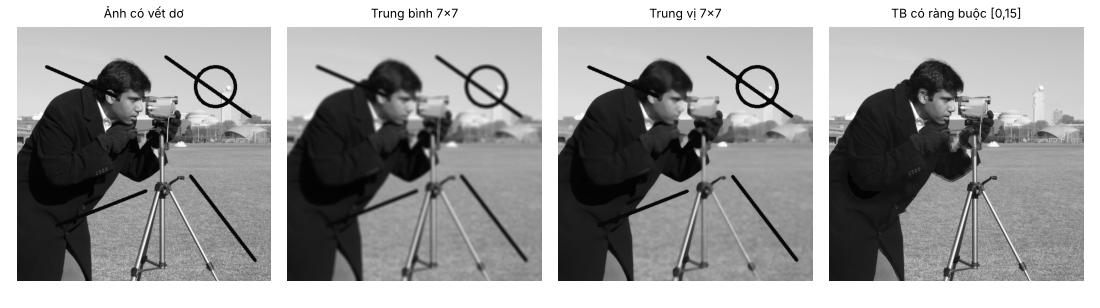
\includegraphics[width=\textwidth]{w6_dirt.png}
\caption{Khử vết dơ (mức xám $8$) bằng lọc trung bình, trung vị và trung bình có ràng buộc.}
\label{fig:w6_dirt}
\end{figure}

\textbf{Hạn chế.} Phương pháp chỉ đúng khi mức xám của vết dơ \emph{không trùng} với mức xám của các chi tiết thật. Trong Hình~\ref{fig:w6_dirt}, một số điểm tối thật của áo khoác (mức xám $\le 15$) cũng bị coi là dơ và bị thay bằng trung bình lân cận, nhưng vì vùng áo vốn tối nên sai số nhỏ. Với ảnh màu hoặc vết dơ có màu đặc trưng, nên xác định điểm dơ bằng ngưỡng trong không gian màu.

% =====================================================================
\subsection{Vì sao bộ lọc trung bình có ràng buộc khử được vết dơ}
\label{subsec:w6_constrained_why}

\textit{Câu hỏi: Giải thích tại sao toán tử trung bình có ràng buộc khử được vết dơ.}

Xét một điểm dơ $(x, y)$ có giá trị $d \in [\min, \max]$, nằm trên nền có giá trị thật là $f_0$. Gọi $\rho$ là tỉ lệ điểm dơ trong cửa sổ.

\textbf{1. Ước lượng không bị nhiễm bẩn.} Bộ lọc trung bình thông thường cho
\begin{equation}
g_{\text{TB}} \approx (1 - \rho)\,f_0 + \rho\,d,
\end{equation}
nên vết dơ chỉ bị pha loãng chứ không biến mất, và với nét rộng ($\rho$ lớn) thì $g_{\text{TB}}$ vẫn gần $d$. Bộ lọc trung vị loại được điểm dơ chỉ khi $\rho < 0{,}5$. Trung bình có ràng buộc loại hẳn các điểm dơ khỏi phép tính, vì $h = 0$ tại các điểm có mức xám trong $[\min, \max]$:
\begin{equation}
g_{\text{RB}} = \frac{1}{|O_{\text{sạch}}|}\sum_{(i, j) \in O_{\text{sạch}}} f(x + i, y + j) \approx f_0,
\end{equation}
với mọi $\rho < 1$, tức chỉ cần \emph{một} điểm sạch trong cửa sổ. Kết quả là ước lượng của nền từ chính các điểm lân cận sạch, đúng với giả thiết ảnh trơn cục bộ.

\textbf{2. Không làm hỏng phần còn lại của ảnh.} Các điểm có giá trị ngoài $[\min, \max]$ được giữ nguyên ($g = f$). Bộ lọc chỉ ``sửa'' đúng các điểm dơ, nên không làm nhòe biên và chi tiết như các bộ lọc tuyến tính.

\textbf{3. Dùng tri thức tiên nghiệm.} Bộ lọc trung bình và trung vị không biết điểm nào là nhiễu, nên phải xử lý mọi điểm như nhau. Trung bình có ràng buộc tận dụng thông tin \emph{biết trước về mức xám của nhiễu} để phát hiện nhiễu trước rồi mới sửa. Đây là ý tưởng chung của các phương pháp lọc ``phát hiện rồi sửa'' (ví dụ lọc trung vị thích nghi chỉ thay các điểm nghi là xung).

\textbf{Điều kiện áp dụng.} (i) Khoảng mức xám của vết dơ tách biệt với mức xám của chi tiết thật, nếu không các chi tiết đó cũng bị xóa; (ii) cửa sổ đủ lớn để luôn có điểm sạch (hoặc lặp nhiều lần); (iii) nền quanh vết dơ trơn, vì nếu vết dơ đè lên biên cạnh thì trung bình các điểm sạch có thể pha trộn hai vùng.

% =====================================================================
\subsection{Toán tử trung bình có trọng số gradient}
\label{subsec:w6_gradient_weighted}

\textit{Câu hỏi: Giải thích công thức của toán tử trung bình có trọng số gradient ở trang 5 của phần bổ sung~\citep{xlav_lec5b}:
\[
h(i, j) = 0{,}5\,\frac{\delta(i, j)}{\sum_{(i', j') \in O \setminus (m, n)} \delta(i', j')}, \qquad h(m, n) = 0{,}5,
\]
\[
\delta(i, j) = \frac{1}{|f(m, n) - f(i, j)|}, \qquad \delta(i, j) = 2 \text{ nếu } f(m, n) = f(i, j),
\]
với $(m, n)$ là điểm đang xét (tâm cửa sổ) và $(i, j)$ là các điểm lân cận.}

\textbf{Ý nghĩa từng thành phần.}
\begin{itemize}
    \item \textbf{$h(m, n) = 0{,}5$}: điểm tâm luôn giữ một nửa trọng số, nên kết quả không bao giờ quá khác giá trị ban đầu; nửa còn lại được chia cho $8$ láng giềng.
    \item \textbf{$\delta(i, j) = 1/|f(m, n) - f(i, j)|$}: trọng số tỉ lệ \emph{nghịch} với chênh lệch mức xám giữa láng giềng và tâm. $|f(m, n) - f(i, j)|$ chính là độ lớn gradient rời rạc theo hướng từ tâm tới láng giềng, nên đây gọi là trọng số nghịch đảo gradient (gradient inverse weighted smoothing~\citep{wang1981gradient}). Láng giềng giống tâm (cùng vùng) đóng góp nhiều; láng giềng khác xa tâm (bên kia biên cạnh) đóng góp rất ít.
    \item \textbf{$\delta = 2$ khi $f(m, n) = f(i, j)$}: tránh chia cho $0$. Với ảnh mức xám nguyên, chênh lệch khác $0$ thì $\ge 1$ nên $\delta \le 1$; quy ước $\delta = 2$ giúp láng giềng giống hệt tâm có trọng số lớn nhất. Do đó $\delta \in (0, 2]$.
    \item \textbf{Chuẩn hóa}: $\sum_{(i, j) \ne (m, n)} h(i, j) = 0{,}5$, cộng với $h(m, n) = 0{,}5$ được tổng bằng $1$, nên độ sáng trung bình được bảo toàn.
\end{itemize}
Kết quả lọc:
\begin{equation}
g(m, n) = 0{,}5\,f(m, n) + 0{,}5\,\frac{\sum_{(i, j)} \delta(i, j)\,f(i, j)}{\sum_{(i, j)} \delta(i, j)}.
\end{equation}

\textbf{Ví dụ.} Tâm $f(m, n) = 100$ nằm sát một biên; $5$ láng giềng cùng vùng có giá trị $98, 101, 102, 100, 99$ và $3$ láng giềng bên kia biên có giá trị $200$. Các $\delta$ tương ứng là $0{,}5;\ 1;\ 0{,}5;\ 2;\ 1$ và $3 \times 0{,}01$, tổng $5{,}03$. Ba điểm $200$ chỉ nhận tổng trọng số $0{,}5 \times 0{,}03/5{,}03 \approx 0{,}003$. Kết quả
\[
g = 0{,}5 \cdot 100 + 0{,}5 \cdot \frac{49 + 101 + 51 + 200 + 99 + 6}{5{,}03} \approx 0{,}5 \cdot 100 + 0{,}5 \cdot 100{,}6 = 100{,}3,
\]
trong khi trung bình $3 \times 3$ cho $1200/9 \approx 133{,}3$: biên bị kéo lệch hơn $33$ mức. Trọng số gradient \emph{làm trơn trong nội bộ vùng nhưng không làm trơn qua biên}.

\textbf{Hạn chế.} Với nhiễu xung, điểm nhiễu ở tâm khác xa mọi láng giềng nên các $\delta$ đều nhỏ và gần bằng nhau. Nửa trọng số còn lại được chia đều, nhưng tâm vẫn giữ $0{,}5$, nên nhiễu chỉ giảm một nửa biên độ. Đây là lý do PSNR với nhiễu muối tiêu chỉ đạt $17{,}77$ dB (Bảng~\ref{tab:w6_filters}). Với nhiễu Gauss, trọng số $1/|\Delta f|$ bị chính nhiễu làm sai lệch, nên hiệu quả khử nhiễu kém hơn bộ lọc Gauss ($24{,}75$ so với $27{,}80$ dB). Phương pháp phù hợp với nhiễu nhỏ khi cần giữ biên.

% =====================================================================
\subsection{Toán tử trung bình dựa trên mặt nạ quay và so sánh với lọc trung vị}
\label{subsec:w6_rotating_mask}

\textit{Câu hỏi: Giải thích ý nghĩa của toán tử trung bình dựa trên mặt nạ quay (trang 6--8 của phần bổ sung~\citep{xlav_lec5b}) và so sánh với phương pháp lọc trung vị.}

\textbf{Giải thuật} (trang 7): tại mỗi điểm $(i, j)$, xét các mặt nạ (vùng con) ``quay'' quanh điểm đó — trong hình ở trang 6 là các mặt nạ $3 \times 3$ có chứa $(i, j)$, đặt ở các vị trí khác nhau trong lân cận $5 \times 5$ (một mặt nạ ở giữa và $8$ mặt nạ lệch về $8$ hướng). Tính phương sai mức xám trong từng mặt nạ, chọn mặt nạ có phương sai nhỏ nhất, gán $g(i, j)$ bằng trung bình của mặt nạ đó~\citep{nagao1979edge}.

\textbf{Ý nghĩa.} Phương sai nhỏ nghĩa là mặt nạ \emph{đồng nhất}, nằm trọn trong một vùng. Gần biên cạnh, mặt nạ ở giữa chứa cả hai vùng nên phương sai lớn; mặt nạ lệch về phía cùng vùng với điểm đang xét có phương sai nhỏ nhất và được chọn. Do đó điểm ảnh chỉ được lấy trung bình với các điểm \emph{cùng phía biên}: nhiễu trong vùng bị làm trơn nhưng biên không bị nhòe, thậm chí được làm sắc thêm. Thực nghiệm biên bậc ở Bảng~\ref{tab:w6_filters} cho thấy biên được giữ nguyên.

\textbf{Công thức phương sai ở trang 8.} Với mặt nạ $R$ có $n$ điểm, trung bình $\mu = \frac{1}{n}\sum_{R} f$:
\begin{equation}
\sigma^2 = \frac{1}{n}\sum_{(i, j) \in R}\big(f(i, j) - \mu\big)^2 = \frac{1}{n}\left[\sum_{(i, j) \in R} f(i, j)^2 - \frac{\big(\sum_{(i, j) \in R} f(i, j)\big)^2}{n}\right].
\end{equation}
\emph{Chứng minh:} khai triển $\sum (f - \mu)^2 = \sum f^2 - 2\mu\sum f + n\mu^2 = \sum f^2 - 2n\mu^2 + n\mu^2 = \sum f^2 - n\mu^2 = \sum f^2 - \frac{(\sum f)^2}{n}$. Dạng thứ hai chỉ cần tổng $\sum f$ và tổng bình phương $\sum f^2$, tính được trong một lần duyệt; với ảnh tích phân của $f$ và $f^2$, phương sai của mọi mặt nạ tính được trong $O(1)$. (Cách tính này có thể mất chính xác số học khi $\sigma^2$ rất nhỏ so với $\mu^2$, nhưng với mức xám 8 bit và số thực 64 bit thì không đáng kể.)

\textbf{So sánh với lọc trung vị.}

\begin{table}[ht]
\centering
\scriptsize
\caption{So sánh toán tử mặt nạ quay và bộ lọc trung vị}
\label{tab:w6_rot_vs_median}
\renewcommand{\arraystretch}{1.3}
\begin{tabularx}{\textwidth}{|p{2.3cm}|X|X|}
\hline
\textbf{Tiêu chí} & \textbf{Mặt nạ quay} & \textbf{Trung vị} \\
\hline
Nguyên lý & Chọn vùng con đồng nhất nhất (phương sai nhỏ nhất) rồi lấy \emph{trung bình} & Lấy \emph{thống kê thứ tự} (giá trị giữa) của cả cửa sổ \\
\hline
Cơ chế giữ biên & Tường minh: tránh lấy mẫu qua biên bằng cách chọn mặt nạ & Ngầm: trung vị luôn là một giá trị có thật thuộc phía chiếm đa số \\
\hline
Nhiễu Gauss & Tốt (trung bình trong vùng đồng nhất): $26{,}71$ dB & Tương đương: $26{,}96$ dB \\
\hline
Nhiễu xung & Khá: $25{,}76$ dB; điểm xung làm tăng phương sai nên mặt nạ chứa nó thường bị loại, nhưng khi mọi mặt nạ đều chứa xung thì xung vẫn bị lấy trung bình & Rất tốt: $29{,}59$ dB \\
\hline
Biên bậc & Giữ nguyên & Giữ nguyên \\
\hline
Chi tiết mảnh, góc & Giữ tốt hơn vì có thể chọn mặt nạ nằm dọc theo chi tiết & Xóa đường mảnh rộng dưới nửa cửa sổ, bo tròn góc \\
\hline
Hiệu ứng phụ & Tạo các mảng đồng màu (hiệu ứng ``tranh sơn dầu''); kết quả có thể nhảy giữa các mặt nạ khi phương sai xấp xỉ nhau & Có thể tạo các mảng phẳng khi lặp nhiều lần \\
\hline
Chi phí & $9$ mặt nạ, mỗi mặt nạ cần trung bình và phương sai; $O(1)$ mỗi mặt nạ với ảnh tích phân & Sắp xếp $9$ giá trị, hoặc lược đồ trượt \\
\hline
\end{tabularx}
\end{table}

Cả hai đều là bộ lọc \emph{phi tuyến giữ biên}. Trung vị phù hợp hơn khi nhiễu chủ yếu là nhiễu xung; mặt nạ quay phù hợp hơn khi nhiễu dạng Gauss và cần giữ biên, góc, chi tiết hình học.

% =====================================================================
\subsection{Bảng thống kê các phương pháp làm trơn và bổ sung bốn phương pháp}
\label{subsec:w6_smoothing_table}

\textit{Câu hỏi: Lập bảng thống kê các phương pháp làm trơn ảnh đã học và bổ sung thêm bốn phương pháp làm trơn khác.}

\clarify{Nhóm hiểu ``bổ sung 4 phương pháp'' là bổ sung $4$ phương pháp ngoài bài giảng. Bảng~\ref{tab:w6_smooth_lecture} thống kê $7$ phương pháp trong bài giảng ($3$ của Bài giảng 5 và $4$ của phần bổ sung), Bảng~\ref{tab:w6_smooth_extra} là $4$ phương pháp bổ sung. Nếu ý câu hỏi là thống kê $4$ phương pháp của phần bổ sung thì Bảng~\ref{tab:w6_smooth_lecture} đã bao gồm.}

\textbf{Toán tử sai số bình phương trung bình tối tiểu} (MMSE, trang 9--10 của phần bổ sung) chưa được giải thích ở các mục trên:
\begin{equation}
g(x, y) = f(x, y) - \frac{\sigma_n^2}{\sigma^2(x, y)}\big[f(x, y) - \bar{f}(x, y)\big],
\end{equation}
với $\sigma_n^2$ là phương sai nhiễu (ước lượng trên vùng đồng nhất), $\bar f(x, y)$ và $\sigma^2(x, y)$ là trung bình và phương sai cục bộ~\citep{lee1980digital}. Ở vùng đồng nhất, $\sigma^2 \approx \sigma_n^2$ nên $g \approx \bar f$ (làm trơn tối đa); gần biên, $\sigma^2 \gg \sigma_n^2$ nên $g \approx f$ (giữ nguyên). Bộ lọc tự động điều chỉnh mức làm trơn theo độ ``bận rộn'' của vùng.

\begin{table}[!htbp]
\centering
\scriptsize
\caption{Thống kê các phương pháp làm trơn trong bài giảng}
\label{tab:w6_smooth_lecture}
\renewcommand{\arraystretch}{1.3}
\begin{tabularx}{\textwidth}{|p{1.7cm}|X|p{2.1cm}|X|p{1.6cm}|}
\hline
\textbf{Phương pháp} & \textbf{Nguyên lý / công thức} & \textbf{Nhiễu phù hợp} & \textbf{Tác động lên biên} & \textbf{Độ phức tạp mỗi điểm} \\
\hline
Trung bình & $g = \sum f(x + i, y + j)/|O|$ & Gauss, đều & Nhòe mạnh & $O(1)$ (tổng trượt) \\
\hline
Gauss & Trung bình trọng số $e^{-(i^2 + j^2)/2\sigma^2}$ & Gauss & Nhòe, mềm hơn trung bình & $O(n)$ (tách được) \\
\hline
Trung vị & $g = \mathrm{med}\{f(x + i, y + j)\}$ & Xung (muối tiêu) & Giữ biên bậc, mất đường mảnh, bo góc & $O(n^2 \log n)$ hoặc $O(n)$ \\
\hline
TB có ràng buộc & Chỉ thay điểm có mức xám trong $[\min, \max]$, chỉ lấy trung bình điểm ngoài $[\min, \max]$ & Vết dơ, nhiễu có khoảng mức xám biết trước & Không ảnh hưởng các điểm sạch & $O(n^2)$ \\
\hline
TB trọng số gradient & Tâm giữ $0{,}5$, láng giềng có trọng số $\propto 1/|f(m, n) - f(i, j)|$ & Gauss biên độ nhỏ & Giữ biên tốt & $O(n^2)$ \\
\hline
Mặt nạ quay & Chọn mặt nạ con có phương sai nhỏ nhất, lấy trung bình mặt nạ đó & Gauss; xung mức độ vừa & Giữ biên, có thể làm sắc biên & $O(9)$ mặt nạ \\
\hline
MMSE & $g = f - \frac{\sigma_n^2}{\sigma^2}(f - \bar f)$ & Gauss (đã biết $\sigma_n^2$), nhiễu đốm & Tự động ít làm trơn gần biên & $O(1)$ (ảnh tích phân) \\
\hline
\end{tabularx}
\end{table}

\begin{table}[!htbp]
\centering
\scriptsize
\caption{Bốn phương pháp làm trơn bổ sung}
\label{tab:w6_smooth_extra}
\renewcommand{\arraystretch}{1.3}
\begin{tabularx}{\textwidth}{|p{1.7cm}|X|p{2.1cm}|X|p{1.6cm}|}
\hline
\textbf{Phương pháp} & \textbf{Nguyên lý / công thức} & \textbf{Nhiễu phù hợp} & \textbf{Tác động lên biên} & \textbf{Độ phức tạp mỗi điểm} \\
\hline
Lọc song phương (bilateral)~\citep{tomasi1998bilateral} & Trọng số là tích của Gauss theo khoảng cách không gian và Gauss theo chênh lệch mức xám: $w = w_s w_r$, \newline $w_s = e^{-(i^2 + j^2)/2\sigma_s^2}$, \newline $w_r = e^{-\Delta f^2/2\sigma_r^2}$, \newline $\Delta f = f(x + i, y + j) - f(x, y)$ & Gauss mức độ vừa & Giữ biên tốt; có thể tạo hiệu ứng bậc thang trên vùng dốc & $O(n^2)$; có giải thuật xấp xỉ nhanh \\
\hline
Khuếch tán dị hướng (Perona--Malik)~\citep{perona1990scale} & Giải phương trình $\partial_t f = \mathrm{div}\big(c(|\nabla f|)\nabla f\big)$ với hệ số khuếch tán $c$ giảm khi gradient lớn; làm trơn lặp nhiều bước & Gauss & Khuếch tán trong vùng, dừng ở biên; làm sắc biên & $O(1)$ mỗi bước, nhiều bước lặp \\
\hline
Trung bình phi cục bộ (NLM)~\citep{buades2005non} & Lấy trung bình các điểm trong vùng tìm kiếm lớn, trọng số theo độ giống nhau giữa \emph{các mảng ảnh} quanh chúng, không theo khoảng cách & Gauss; mạnh với ảnh có kết cấu lặp & Giữ biên và kết cấu tốt & $O(S^2 P^2)$, rất tốn \\
\hline
BM3D~\citep{dabov2007image} & Gom các mảng giống nhau thành khối 3D, biến đổi miền tần số 3D, co ngưỡng hệ số, biến đổi ngược và gộp kết quả (hai giai đoạn) & Gauss (biết $\sigma$) & Giữ biên và chi tiết rất tốt; là mức tham chiếu của khử nhiễu cổ điển & Cao \\
\hline
\end{tabularx}
\end{table}

\textbf{Hướng phát triển.} Các phương pháp học sâu như DnCNN~\citep{zhang2017beyond} học trực tiếp ánh xạ từ ảnh nhiễu sang nhiễu (học phần dư) và vượt BM3D khi có dữ liệu huấn luyện phù hợp; xu hướng hiện nay là các mạng khử nhiễu không cần ảnh sạch và mô hình khuếch tán.

% =====================================================================
\subsection{Nguyên lý phát hiện biên cạnh}
\label{subsec:w6_edge_principle}

\textit{Câu hỏi: Trình bày nguyên lý phát hiện biên cạnh.}

\textbf{Biên cạnh là gì.} Biên cạnh là tập các điểm ảnh tại đó \emph{mức xám thay đổi đột ngột}. Sự thay đổi này thường do ranh giới giữa hai đối tượng, sự gián đoạn độ sâu, sự thay đổi hướng bề mặt, thay đổi tính chất phản xạ (màu, vật liệu) hoặc bóng đổ~\citep{xlav_lec6}. Biên mang phần lớn thông tin hình dạng của ảnh: ảnh biên ở trang 5--6 của bài giảng vẫn đủ để nhận ra ngôi nhà dù chỉ còn vài phần trăm số điểm ảnh. Trang 9 phân loại biên theo hình dạng mặt cắt: biên bậc (step), biên dốc (ramp), biên đường (line) và biên mái nhà (roof).

\textbf{Biên được mô tả bởi đạo hàm.} Sự thay đổi đột ngột của hàm $f$ được đo bằng đạo hàm. Với biên dốc một chiều (trang 8):
\begin{itemize}
    \item \textbf{Đạo hàm bậc nhất} $f'$ đạt \emph{cực trị} tại tâm biên. Trong 2 chiều, vector gradient $\nabla f = (f_x, f_y)^T$ cho biết độ lớn $e = \|\nabla f\|$ (độ mạnh của biên) và hướng $\phi$ (hướng thay đổi nhanh nhất, vuông góc với hướng đường biên — trang 7, 10).
    \item \textbf{Đạo hàm bậc hai} $f''$ \emph{đổi dấu (qua $0$)} tại tâm biên. Trong 2 chiều dùng toán tử Laplace $\nabla^2 f = f_{xx} + f_{yy}$ và tìm các điểm qua $0$.
\end{itemize}

\textbf{Quy trình chung.}
\begin{enumerate}
    \item \textbf{Làm trơn} để giảm nhiễu, vì đạo hàm khuếch đại nhiễu (Mục~\ref{subsec:w6_derivative_difficulty}).
    \item \textbf{Lấy đạo hàm rời rạc} bằng các mặt nạ: sai phân, Roberts, Prewitt, Sobel, Frei-Chen (bậc một); Laplace, LoG (bậc hai).
    \item \textbf{Phát hiện}: phân ngưỡng độ lớn gradient, hoặc tìm điểm qua $0$ có độ dốc đủ lớn.
    \item \textbf{Định vị và làm mảnh}: giữ lại các điểm cực đại theo hướng gradient (non-maximum suppression) để biên chỉ rộng $1$ điểm.
    \item \textbf{Liên kết biên}: nối các điểm biên thành đường, loại các đoạn ngắn rời rạc (ngưỡng trễ trong phương pháp Canny~\citep{canny1986computational}).
\end{enumerate}
Một bộ phát hiện biên tốt cần thỏa ba tiêu chí của Canny: phát hiện đúng (ít bỏ sót, ít biên giả), định vị chính xác (gần tâm biên thật) và đáp ứng duy nhất (mỗi biên chỉ cho một đường).

% =====================================================================
\subsection{Khó khăn của phương pháp dựa trên đạo hàm bậc nhất; đặc điểm của đạo hàm bậc hai}
\label{subsec:w6_derivative_difficulty}

\textit{Câu hỏi: Nếu dựa trên đạo hàm bậc nhất để xác định biên cạnh thì sẽ gặp những khó khăn gì? So với đạo hàm bậc nhất, đạo hàm bậc hai có gì đặc biệt?}

\textbf{Khó khăn của đạo hàm bậc nhất.}
\begin{enumerate}
    \item \textbf{Nhạy với nhiễu.} Phép lấy đạo hàm là bộ lọc thông cao (đáp ứng tần số $\propto |\omega|$), khuếch đại chính các tần số cao nơi nhiễu chiếm ưu thế. Với nhiễu độc lập phương sai $\sigma^2$, sai phân $f(x, y) - f(x - 1, y)$ có phương sai nhiễu $2\sigma^2$, trong khi ở vùng đồng nhất tín hiệu đạo hàm bằng $0$. Do đó phải làm trơn trước, mà làm trơn lại làm biên nhòe.
    \item \textbf{Chọn ngưỡng.} Gradient chỉ cho một ``độ mạnh'', ta phải chọn ngưỡng $T$ để quyết định điểm biên. Ngưỡng thấp thì nhận nhiều biên giả từ nhiễu và kết cấu; ngưỡng cao thì biên bị đứt, mất các biên có độ tương phản thấp. Một ngưỡng chung khó phù hợp với mọi vùng của ảnh có độ sáng không đều.
    \item \textbf{Biên dày, định vị kém.} Trên biên dốc, gradient khác $0$ trên toàn bộ dốc, không chỉ tại tâm. Theo trang 16--17 và 21--22 của bài giảng: với biên dốc độ cao $h$, sai phân lùi cho chuỗi $0\ 0\ h/2\ h/2\ 0\ 0$ (hai điểm, tâm biên nằm giữa hai điểm ảnh), sai phân trung tâm cho $0\ h/2\ h\ h/2\ 0$ (ba điểm). Sau khi phân ngưỡng, biên dày nhiều điểm ảnh, phải làm mảnh bằng non-maximum suppression.
    \item \textbf{Phụ thuộc hướng.} Gradient có hai thành phần, phải tính bằng hai mặt nạ. Các mặt nạ rời rạc không đẳng hướng hoàn toàn: độ lớn đo được thay đổi theo hướng biên (trang 28--29: với biên chéo, Prewitt cho $0{,}94h$, Sobel cho $1{,}06h$, chỉ Frei-Chen cho đúng $h$).
    \item \textbf{Cần bước tìm cực đại.} Bản chất biên là cực đại của $|f'|$, mà tìm cực đại 2 chiều theo hướng gradient phức tạp hơn tìm điểm đổi dấu.
\end{enumerate}

\textbf{Đặc điểm của đạo hàm bậc hai.}
\begin{itemize}
    \item \textbf{Định vị chính xác, biên mảnh.} Tâm biên tương ứng với điểm \emph{qua $0$} của $f''$. Điểm qua $0$ xác định duy nhất, kể cả trên biên dốc rộng, và có thể ước lượng ở độ chính xác dưới điểm ảnh bằng nội suy. Ví dụ ở trang 44: Laplace của biên dốc cho $0\ \ {-3h/8}\ \ 3h/8\ \ 0$, tâm biên nằm ngay giữa hai giá trị trái dấu. Không cần ngưỡng để quyết định ``độ dày''.
    \item \textbf{Đẳng hướng.} Laplace $\nabla^2 f = f_{xx} + f_{yy}$ là toán tử vô hướng, bất biến với phép quay: chỉ cần \emph{một} mặt nạ cho mọi hướng biên.
    \item \textbf{Đường biên khép kín.} Tập điểm qua $0$ của một hàm trơn là các đường cong liên tục, nên biên LoG thường khép kín.
    \item \textbf{Dấu cho biết phía sáng/tối}: $f'' > 0$ ở phía tối, $f'' < 0$ ở phía sáng của biên.
    \item \textbf{Nhưng}: còn nhạy với nhiễu hơn đạo hàm bậc nhất (đáp ứng tần số $\propto \omega^2$); không cho hướng biên; vùng đồng nhất có nhiễu cũng có vô số điểm qua $0$ (Hình~\ref{fig:w6_edges}: Laplace không làm trơn cho $25{,}5\%$ điểm biên, phần lớn là biên giả trên bãi cỏ), nên bắt buộc phải làm trơn (LoG) và chỉ nhận các điểm qua $0$ có độ dốc lớn; với biên đường (line) cho đáp ứng kép.
\end{itemize}

% =====================================================================
\subsection{Ý nghĩa hình học của vector gradient và phân biệt với vector pháp tuyến của mặt \texorpdfstring{$z = f(x, y)$}{z = f(x, y)}}
\label{subsec:w6_gradient_geometry}

\textit{Câu hỏi: Trang 10 của Bài giảng 6 định nghĩa vector gradient $(\nabla f)(x, y) = [\partial f/\partial x\ \ \partial f/\partial y]^T = [f_x\ \ f_y]^T$, độ lớn biên $e(x, y) = \big(f_x^2 + f_y^2\big)^{1/2}$ và hướng $\phi(x, y)$~\citep{xlav_lec6}. Hãy nêu ý nghĩa hình học của vector gradient của $f$, và phân biệt vector gradient của $f$ với vector pháp tuyến của mặt cong $z = f(x, y)$.}

\textbf{Ghi chú về công thức hướng.} Slide ghi $\phi(x, y) = \arctan(f_x\ f_y)$; công thức đúng là $\phi = \arctan(f_y / f_x)$, trong cài đặt nên dùng $\operatorname{atan2}(f_y, f_x)$ để có góc trong $(-\pi, \pi]$ và tránh chia cho $0$.

\textbf{Ý nghĩa hình học của $\nabla f$.} Xem ảnh là một hàm độ cao trên mặt phẳng ảnh. Đạo hàm theo hướng của vector đơn vị $\mathbf{u} = (\cos\theta, \sin\theta)$ là
\begin{equation}
D_{\mathbf{u}} f = f_x\cos\theta + f_y\sin\theta = \nabla f \cdot \mathbf{u} = \|\nabla f\|\cos(\theta - \phi).
\end{equation}
Từ đó:
\begin{enumerate}
    \item \textbf{Hướng}: $D_{\mathbf{u}} f$ lớn nhất khi $\theta = \phi$. Vector gradient chỉ \emph{hướng mức xám tăng nhanh nhất}, từ vùng tối sang vùng sáng.
    \item \textbf{Độ lớn}: giá trị lớn nhất đó bằng $e = \|\nabla f\|$, là \emph{tốc độ thay đổi lớn nhất} của mức xám tại điểm đang xét, tức độ mạnh của biên.
    \item \textbf{Vuông góc với đường đồng mức}: theo hướng $\theta = \phi \pm 90^\circ$ thì $D_{\mathbf{u}} f = 0$, mức xám không đổi. Đường đồng mức $f(x, y) = \text{const}$ (đường biên) vuông góc với $\nabla f$. Đây là lý do trang 7 vẽ ``gradient $\Psi$'' vuông góc với ``edge direction $\Phi$'': hướng biên $= \phi \pm 90^\circ$.
\end{enumerate}
Lưu ý $\nabla f$ là vector \emph{2 chiều, nằm trong mặt phẳng ảnh} $Oxy$, và bằng vector $\mathbf{0}$ ở vùng đồng nhất.

\textbf{Vector pháp tuyến của mặt $z = f(x, y)$.} Xem ảnh như một mặt cong trong không gian 3 chiều $(x, y, z)$. Mặt này là tập mức $0$ của hàm $F(x, y, z) = f(x, y) - z$, nên vector pháp tuyến là gradient 3 chiều của $F$:
\begin{equation}
\mathbf{n} = \nabla F = (f_x,\ f_y,\ -1)^T, \qquad \hat{\mathbf{n}} = \frac{(f_x, f_y, -1)}{\sqrt{1 + f_x^2 + f_y^2}}.
\end{equation}

\textbf{Phân biệt và liên hệ.}
\begin{itemize}
    \item \emph{Không gian}: $\nabla f \in \mathbb{R}^2$, nằm trong mặt phẳng ảnh; $\mathbf{n} \in \mathbb{R}^3$, vuông góc với mặt cong độ sáng.
    \item \emph{Vùng phẳng}: $\nabla f = \mathbf{0}$ (không xác định hướng) trong khi $\mathbf{n} = (0, 0, -1)$ vẫn là vector khác $0$, hướng thẳng đứng.
    \item \emph{Ý nghĩa}: $\nabla f$ là hướng ``leo dốc'' nhanh nhất \emph{trên mặt đất} (mặt phẳng ảnh); $\mathbf{n}$ là hướng vuông góc với ``sườn đồi''.
    \item \emph{Liên hệ}: hình chiếu của $-\mathbf{n}$ (hoặc của $\mathbf{n}$, đổi dấu) lên mặt phẳng $Oxy$ chính là $\pm\nabla f$, nên hai vector có cùng phương ngang. Góc nghiêng $\alpha$ giữa $\mathbf{n}$ và trục $Oz$ thỏa $\tan\alpha = \|\nabla f\|$: biên càng mạnh thì sườn đồi càng dốc, pháp tuyến càng nghiêng.
\end{itemize}
Trong phát hiện biên ta dùng $\nabla f$ (độ lớn và hướng trong mặt phẳng ảnh). Vector pháp tuyến 3 chiều dùng trong các bài toán khác như chiếu sáng, tái tạo hình dạng từ bóng đổ (shape from shading) và bản đồ pháp tuyến trong đồ họa máy tính.

% =====================================================================
\subsection{Giải thuật xác định biên cạnh trong ảnh}
\label{subsec:w6_edge_algorithm}

\textit{Câu hỏi: Viết giải thuật xác định biên cạnh trong ảnh.}

Giải thuật~\ref{alg:w6_edge} dựa trên gradient, gồm các bước của phương pháp Canny trong bài giảng (trang 52--58)~\citep{xlav_lec6,canny1986computational}: làm trơn Gauss, tính gradient bằng Sobel, loại bỏ điểm không cực đại theo hướng gradient và phân ngưỡng trễ. Bỏ bước 4--5 và thay bằng $E \gets [e \ge T]$ ta được bộ phát hiện biên gradient đơn giản nhất.

\begin{algorithm}[ht]
\caption{Phát hiện biên cạnh dựa trên gradient}
\label{alg:w6_edge}
\begin{algorithmic}[1]
\Require Ảnh xám $f$ kích thước $N \times M$; $\sigma$; ngưỡng thấp $t_0$, ngưỡng cao $t_1$ ($t_0 < t_1$)
\Ensure Ảnh biên nhị phân $E$
\State $f_s \gets f * G_\sigma$ \Comment{1. làm trơn Gauss (Mục~\ref{subsec:w6_gauss_kernels})}
\State $f_x \gets f_s \otimes W_x$, \quad $f_y \gets f_s \otimes W_y$ \Comment{2. mặt nạ Sobel, trang 38}
\For{mỗi điểm $(x, y)$}
    \State $e(x, y) \gets \sqrt{f_x^2 + f_y^2}$; \quad $\phi(x, y) \gets \operatorname{atan2}(f_y, f_x)$
\EndFor
\For{mỗi điểm $(x, y)$ có $e(x, y) > 0$} \Comment{3. non-maximum suppression}
    \State Làm tròn $\phi$ về một trong $4$ hướng $0^\circ, 45^\circ, 90^\circ, 135^\circ$; gọi $p_1$, $p_2$ là hai láng giềng theo hướng đó
    \If{$e(p_1) > e(x, y)$ \textbf{or} $e(p_2) > e(x, y)$} \State đánh dấu xóa $(x, y)$ \EndIf
\EndFor
\State Gán $e(x, y) \gets 0$ cho mọi điểm bị đánh dấu xóa
\State $E(x, y) \gets 1$ nếu $e(x, y) \ge t_1$, ngược lại $0$ \Comment{4. biên mạnh}
\Repeat \Comment{5. ngưỡng trễ: nối biên yếu vào biên mạnh}
    \For{mỗi điểm $(x, y)$ có $t_0 \le e(x, y) < t_1$ và $E(x, y) = 0$}
        \If{có láng giềng $8$ hướng $q$ với $E(q) = 1$} \State $E(x, y) \gets 1$ \EndIf
    \EndFor
\Until{$E$ không thay đổi}
\State \Return $E$
\end{algorithmic}
\end{algorithm}

\textbf{Độ phức tạp.} Các bước 1--4 tốn $O(NM)$ với mặt nạ kích thước cố định. Bước 5 nếu cài bằng lặp như trên có thể tốn nhiều vòng; cài bằng loang (BFS/DFS) từ các điểm biên mạnh thì chỉ tốn $O(NM)$.

\textbf{Kết quả.} Hình~\ref{fig:w6_edges} so sánh trên ảnh \texttt{camera}: phân ngưỡng $|\nabla f| \ge 30$ (Sobel, không làm mảnh) cho $10{,}6\%$ điểm biên, biên dày và nhiều điểm biên trên bãi cỏ; Laplace 8 hướng không làm trơn cho $25{,}5\%$; LoG ($\sigma = 1{,}4$) cho biên mảnh, khép kín, $7{,}2\%$ điểm biên (Mục~\ref{subsec:w6_laplace_algorithm}).

\begin{figure}[ht]
\centering
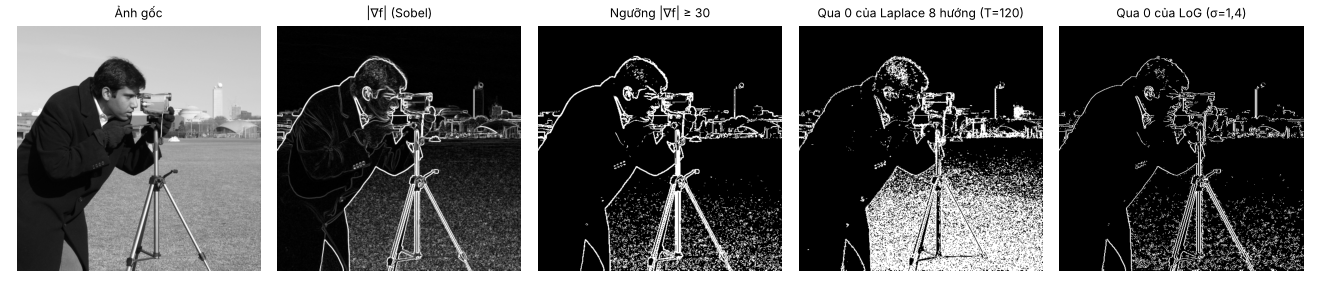
\includegraphics[width=\textwidth]{w6_edges.png}
\caption{Phát hiện biên trên ảnh \texttt{camera}: độ lớn gradient Sobel, phân ngưỡng gradient, điểm qua $0$ của Laplace 8 hướng (ngưỡng độ dốc $T = 120$) và của LoG $9 \times 9$, $\sigma = 1{,}4$ (ngưỡng $T = 6$).}
\label{fig:w6_edges}
\end{figure}

% =====================================================================
\subsection{Chứng minh dạng mở rộng 8 hướng của toán tử Laplace}
\label{subsec:w6_laplace_8dir}

\textit{Câu hỏi: Bài giảng (trang 40--43) cho toán tử Laplace rời rạc dạng $4$ hướng $\begin{bmatrix} 0 & 1 & 0 \\ 1 & -4 & 1 \\ 0 & 1 & 0 \end{bmatrix}$ và dạng mở rộng $8$ hướng $\begin{bmatrix} 1 & 1 & 1 \\ 1 & -8 & 1 \\ 1 & 1 & 1 \end{bmatrix}$~\citep{xlav_lec6}. Hãy chứng minh rằng chập ảnh với mặt nạ $8$ hướng cũng cho một xấp xỉ của toán tử Laplace $\nabla^2 f = f_{xx} + f_{yy}$.}

\textbf{Bước 1: dạng 4 hướng.} Khai triển Taylor theo $x$ với bước lưới $1$:
\begin{equation}
f(x \pm 1, y) = f \pm f_x + \tfrac{1}{2}f_{xx} \pm \tfrac{1}{6}f_{xxx} + \tfrac{1}{24}f_{xxxx} + \ldots
\end{equation}
Cộng hai đẳng thức: $f(x + 1, y) + f(x - 1, y) - 2f = f_{xx} + \tfrac{1}{12}f_{xxxx} + \ldots$. Tương tự theo $y$. Cộng lại:
\begin{equation}
f(x + 1, y) + f(x - 1, y) + f(x, y + 1) + f(x, y - 1) - 4f(x, y) = \nabla^2 f + O(h^2),
\end{equation}
đúng là công thức trang 40 và mặt nạ $4$ hướng ở trang 42.

\textbf{Bước 2: hai hướng chéo.} Xét hệ trục quay $45^\circ$ với các vector đơn vị $\mathbf{u} = \frac{1}{\sqrt 2}(1, 1)$ và $\mathbf{v} = \frac{1}{\sqrt 2}(1, -1)$. Điểm $(x + 1, y + 1)$ cách $(x, y)$ một khoảng $\sqrt 2$ theo hướng $\mathbf{u}$, nên tương tự bước 1 với bước lưới $\sqrt 2$:
\begin{equation}
f(x + 1, y + 1) + f(x - 1, y - 1) - 2f = (\sqrt 2)^2 f_{uu} + O(h^4) = 2f_{uu} + O(h^4),
\end{equation}
và tương tự $f(x + 1, y - 1) + f(x - 1, y + 1) - 2f = 2f_{vv} + O(h^4)$. Vì Laplace \emph{bất biến với phép quay} hệ trục ($f_{uu} + f_{vv} = f_{xx} + f_{yy}$, kiểm tra trực tiếp: $f_{uu} = \tfrac12(f_{xx} + 2f_{xy} + f_{yy})$, $f_{vv} = \tfrac12(f_{xx} - 2f_{xy} + f_{yy})$, cộng lại thì $f_{xy}$ triệt tiêu), mặt nạ chéo
\begin{equation}
L_{\times} = \begin{bmatrix} 1 & 0 & 1 \\ 0 & -4 & 0 \\ 1 & 0 & 1 \end{bmatrix}
\quad \text{cho} \quad L_{\times} \otimes f = 2(f_{uu} + f_{vv}) + O(h^2) = 2\nabla^2 f + O(h^2).
\end{equation}

\textbf{Bước 3: cộng hai mặt nạ.} Mặt nạ $8$ hướng chính là tổng mặt nạ $4$ hướng và mặt nạ chéo:
\begin{equation}
L_8 = \begin{bmatrix} 0 & 1 & 0 \\ 1 & -4 & 1 \\ 0 & 1 & 0 \end{bmatrix} + \begin{bmatrix} 1 & 0 & 1 \\ 0 & -4 & 0 \\ 1 & 0 & 1 \end{bmatrix} = \begin{bmatrix} 1 & 1 & 1 \\ 1 & -8 & 1 \\ 1 & 1 & 1 \end{bmatrix},
\end{equation}
nên theo tính tuyến tính của phép chập:
\begin{equation}
L_8 \otimes f = \nabla^2 f + 2\nabla^2 f + O(h^2) = 3\,\nabla^2 f + O(h^2).
\end{equation}

\textbf{Kiểm tra trực tiếp bằng Taylor 2 chiều.} $f(x + i, y + j) = f + i f_x + j f_y + \tfrac12(i^2 f_{xx} + 2ij f_{xy} + j^2 f_{yy}) + O(h^3)$. Cộng $8$ láng giềng $(i, j) \in \{-1, 0, 1\}^2 \setminus \{(0, 0)\}$: $\sum i = \sum j = \sum ij = 0$ (các số hạng bậc nhất và $f_{xy}$ triệt tiêu do đối xứng), $\sum i^2 = \sum j^2 = 6$. Các số hạng bậc ba cũng triệt tiêu vì đối xứng tâm. Vậy
\begin{equation}
\sum_{(i, j) \ne (0, 0)} f(x + i, y + j) - 8f(x, y) = \tfrac12(6 f_{xx} + 6 f_{yy}) + O(h^4) = 3\,\nabla^2 f + O(h^4). \qquad \square
\end{equation}

\textbf{Nhận xét.} Mặt nạ $8$ hướng là Laplace nhân hệ số $3$; hệ số này không ảnh hưởng tới vị trí điểm qua $0$, chỉ ảnh hưởng tới ngưỡng. Mặt nạ $8$ hướng dùng cả thông tin hai đường chéo nên \emph{gần đẳng hướng hơn} mặt nạ $4$ hướng (mặt nạ $4$ hướng phản ứng yếu hơn với biên chéo), nhưng cũng nhạy với nhiễu hơn vì dùng nhiều điểm hơn với hệ số tâm lớn hơn. Vì hai mặt nạ đối xứng tâm, chập và tương quan cho cùng kết quả. Các tổ hợp khác như $\frac{1}{6}\big(4 L_4 + L_\times\big)$ cho xấp xỉ có sai số bậc cao đẳng hướng hơn.

% =====================================================================
\subsection{Giải thuật phát hiện biên cạnh dựa trên toán tử Laplace (dò điểm qua 0)}
\label{subsec:w6_laplace_algorithm}

\textit{Câu hỏi: Viết giải thuật phát hiện biên cạnh dựa trên toán tử Laplace bằng cách dò tìm những vị trí có sự chuyển tiếp giữa giá trị âm và giá trị dương (điểm qua $0$).}

\textbf{Ý tưởng.} Tại tâm biên, $\nabla^2 f$ đổi dấu (Mục~\ref{subsec:w6_derivative_difficulty}). Ta tính ảnh Laplace $L = f \otimes \text{Laplace}$ rồi đánh dấu các điểm mà $L$ đổi dấu so với một láng giềng. Có hai điểm cần lưu ý: (i) giá trị đúng bằng $0$ thường xuất hiện ở vùng đồng nhất và trên cạnh dốc thẳng, nên chỉ xét cặp \emph{trái dấu ngặt} ($L_1 L_2 < 0$), hoặc bộ ba $(+, 0, -)$; (ii) nhiễu tạo ra rất nhiều điểm qua $0$ yếu, nên chỉ nhận điểm qua $0$ có \emph{độ dốc} $|L_1 - L_2| \ge T$. Để giảm nhiễu, nên làm trơn bằng Gauss trước, tức dùng LoG (Mục~\ref{subsec:w6_log_kernels}).

\begin{algorithm}[ht]
\caption{Phát hiện biên bằng điểm qua $0$ của Laplace / LoG}
\label{alg:w6_zero_crossing}
\begin{algorithmic}[1]
\Require Ảnh xám $f$ kích thước $N \times M$; mặt nạ $K$ (Laplace $4$/$8$ hướng hoặc LoG); ngưỡng độ dốc $T$
\Ensure Ảnh biên nhị phân $E$
\State $L \gets f \otimes K$ \Comment{tính bằng số thực, giữ dấu}
\State $E \gets 0$
\For{$y = 0, \ldots, N - 1$}
    \For{$x = 0, \ldots, M - 1$}
        \For{$(d_x, d_y) \in \{(1, 0), (0, 1), (1, 1), (-1, 1)\}$} \Comment{phải, dưới, hai đường chéo}
            \State $(x_2, y_2) \gets (x + d_x, y + d_y)$; \textbf{nếu} ngoài ảnh \textbf{thì} bỏ qua
            \If{$L(x, y) \cdot L(x_2, y_2) < 0$ \textbf{and} $|L(x, y) - L(x_2, y_2)| \ge T$}
                \State $E(x, y) \gets 1$ \Comment{có thể chọn đánh dấu điểm có $|L|$ nhỏ hơn để biên nằm sát tâm}
            \EndIf
        \EndFor
        \If{$L(x, y) = 0$ \textbf{and} $\exists (d_x, d_y)$: $L(x - d_x, y - d_y) \cdot L(x + d_x, y + d_y) < 0$ và $|L(x - d_x, y - d_y) - L(x + d_x, y + d_y)| \ge T$}
            \State $E(x, y) \gets 1$ \Comment{trường hợp $(+, 0, -)$}
        \EndIf
    \EndFor
\EndFor
\State \Return $E$
\end{algorithmic}
\end{algorithm}

Giải thuật tốn $O(NM \cdot k^2)$ cho bước chập với mặt nạ $k \times k$ và $O(NM)$ cho bước dò. Hàm \texttt{zero\_crossings} trong \texttt{XLAV/code/w6\_lib.py} cài đặt phần trái dấu ngặt. Hình~\ref{fig:w6_edges} cho thấy với Laplace $3 \times 3$ không làm trơn, dù đã đặt ngưỡng độ dốc $T = 120$, vẫn còn rất nhiều điểm qua $0$ do nhiễu và kết cấu (cỏ); với LoG $\sigma = 1{,}4$, biên mảnh, liên tục và sạch hơn hẳn.

% =====================================================================
\subsection{Hệ số của bộ lọc Laplace of Gaussian kích thước \texorpdfstring{$3$, $5$, $7$}{3, 5, 7}}
\label{subsec:w6_log_kernels}

\textit{Câu hỏi: Xác định các hệ số của bộ lọc Laplace of Gaussian (LoG) với kích thước $3 \times 3$, $5 \times 5$, $7 \times 7$.}

\textbf{Công thức.} Do tính tuyến tính, $\nabla^2(G_\sigma * f) = (\nabla^2 G_\sigma) * f$ (trang 49): thay vì làm trơn rồi lấy Laplace, ta chập một lần với nhân $\nabla^2 G_\sigma$. Với $G(x, y) = \frac{1}{2\pi\sigma^2}e^{-r^2/2\sigma^2}$, $r^2 = x^2 + y^2$:
\begin{equation}
G_{xx} = \frac{1}{2\pi\sigma^2}\left(\frac{x^2}{\sigma^4} - \frac{1}{\sigma^2}\right)e^{-\frac{r^2}{2\sigma^2}}
\;\Rightarrow\;
\nabla^2 G = G_{xx} + G_{yy} = \frac{1}{\pi\sigma^4}\left(\frac{r^2}{2\sigma^2} - 1\right)e^{-\frac{r^2}{2\sigma^2}},
\end{equation}
trùng với công thức trang 49 (dạng ``mũ Mexico'' lộn ngược: âm ở tâm, đổi dấu tại $r = \sqrt 2\,\sigma$, dương ở vành ngoài).

\textbf{Chọn $\sigma$ và hiệu chỉnh.} Để mặt nạ chứa được cả phần âm ở tâm và một phần vành dương, bán kính đổi dấu $\sqrt 2\sigma$ phải nhỏ hơn bán kính $r_{\max} = (n - 1)/2$ của cửa sổ. Nhóm chọn $\sigma = 0{,}5;\ 0{,}8;\ 1{,}1$ cho $n = 3, 5, 7$ (bán kính đổi dấu $0{,}71;\ 1{,}13;\ 1{,}56$). Sau khi lấy mẫu công thức tại các điểm nguyên, ta \emph{trừ đi giá trị trung bình} để tổng các hệ số bằng $0$. Đây là điều kiện bắt buộc của mọi toán tử đạo hàm: vùng có độ sáng không đổi phải cho đáp ứng $0$; nếu bỏ qua, phần đuôi bị cắt cụt làm tổng khác $0$ và vùng phẳng sinh ra đáp ứng giả. Hệ số nguyên thu được bằng cách co giãn cho hệ số tâm bằng $-40$, làm tròn, rồi chỉnh hệ số tâm để tổng đúng bằng $0$.

$n = 3$, $\sigma = 0{,}5$:
\[
\mathrm{LoG}_3 = \begin{bmatrix} 0{,}4150 & 0{,}8244 & 0{,}4150 \\ 0{,}8244 & -4{,}9578 & 0{,}8244 \\ 0{,}4150 & 0{,}8244 & 0{,}4150 \end{bmatrix}
\approx \begin{bmatrix} 3 & 7 & 3 \\ 7 & -40 & 7 \\ 3 & 7 & 3 \end{bmatrix}.
\]
Với $3 \times 3$, LoG chỉ còn là một mặt nạ Laplace có trọng số giữa dạng $4$ hướng và $8$ hướng; tác dụng làm trơn gần như không có.

$n = 5$, $\sigma = 0{,}8$:
\[
\mathrm{LoG}_5 = \begin{bmatrix}
0{,}0093 & 0{,}0469 & 0{,}0740 & 0{,}0469 & 0{,}0093 \\
0{,}0469 & 0{,}0931 & -0{,}0764 & 0{,}0931 & 0{,}0469 \\
0{,}0740 & -0{,}0764 & -0{,}7757 & -0{,}0764 & 0{,}0740 \\
0{,}0469 & 0{,}0931 & -0{,}0764 & 0{,}0931 & 0{,}0469 \\
0{,}0093 & 0{,}0469 & 0{,}0740 & 0{,}0469 & 0{,}0093
\end{bmatrix},
\]
\[
\mathrm{LoG}_5 \approx \begin{bmatrix}
0 & 2 & 4 & 2 & 0 \\ 2 & 5 & -4 & 5 & 2 \\ 4 & -4 & -36 & -4 & 4 \\ 2 & 5 & -4 & 5 & 2 \\ 0 & 2 & 4 & 2 & 0
\end{bmatrix}.
\]

$n = 7$, $\sigma = 1{,}1$:
\[
\mathrm{LoG}_7 = \begin{bmatrix}
0{,}0012 & 0{,}0048 & 0{,}0113 & 0{,}0148 & 0{,}0113 & 0{,}0048 & 0{,}0012 \\
0{,}0048 & 0{,}0188 & 0{,}0298 & 0{,}0276 & 0{,}0298 & 0{,}0188 & 0{,}0048 \\
0{,}0113 & 0{,}0298 & -0{,}0161 & -0{,}0840 & -0{,}0161 & 0{,}0298 & 0{,}0113 \\
0{,}0148 & 0{,}0276 & -0{,}0840 & -0{,}2170 & -0{,}0840 & 0{,}0276 & 0{,}0148 \\
0{,}0113 & 0{,}0298 & -0{,}0161 & -0{,}0840 & -0{,}0161 & 0{,}0298 & 0{,}0113 \\
0{,}0048 & 0{,}0188 & 0{,}0298 & 0{,}0276 & 0{,}0298 & 0{,}0188 & 0{,}0048 \\
0{,}0012 & 0{,}0048 & 0{,}0113 & 0{,}0148 & 0{,}0113 & 0{,}0048 & 0{,}0012
\end{bmatrix},
\]
\[
\mathrm{LoG}_7 \approx \begin{bmatrix}
0 & 1 & 2 & 3 & 2 & 1 & 0 \\
1 & 3 & 5 & 5 & 5 & 3 & 1 \\
2 & 5 & -3 & -15 & -3 & 5 & 2 \\
3 & 5 & -15 & -36 & -15 & 5 & 3 \\
2 & 5 & -3 & -15 & -3 & 5 & 2 \\
1 & 3 & 5 & 5 & 5 & 3 & 1 \\
0 & 1 & 2 & 3 & 2 & 1 & 0
\end{bmatrix}.
\]

\textbf{Lưu ý.} (i) Nhiều tài liệu dùng $-\nabla^2 G$ (tâm dương); đổi dấu toàn bộ mặt nạ không làm thay đổi vị trí điểm qua $0$. (ii) Mặt nạ $5 \times 5$ quen thuộc trong sách $\begin{bmatrix}0&0&1&0&0\\0&1&2&1&0\\1&2&-16&2&1\\0&1&2&1&0\\0&0&1&0&0\end{bmatrix}$ ứng với $\sigma$ nhỏ hơn ($\approx 0{,}5$--$0{,}6$), khi đó cả $4$ láng giềng gần đều dương. (iii) $\sigma$ càng lớn thì càng ít nhiễu nhưng biên nhỏ bị mất và các góc bị bo tròn; cửa sổ nên có kích thước khoảng $6\sigma$--$8\sigma$ để không cắt cụt quá nhiều (vì vậy Hình~\ref{fig:w6_edges} dùng mặt nạ $9 \times 9$ cho $\sigma = 1{,}4$). Mã tính: hàm \texttt{log\_kernel(n, sigma)} trong \texttt{XLAV/code/w6\_lib.py}.

% =====================================================================
\subsection{Bảng thống kê các phương pháp phát hiện biên cạnh}
\label{subsec:w6_edge_table}

\textit{Câu hỏi: Lập bảng thống kê các phương pháp phát hiện biên cạnh theo các tiêu chí: nguyên lý, phương pháp, khả năng phát hiện biên cạnh, phản ứng phụ (với nhiễu) và độ phức tạp tính toán.}

\begin{table}[!htbp]
\centering
\scriptsize
\caption{Thống kê các phương pháp phát hiện biên cạnh (Bài giảng 6)}
\label{tab:w6_edge_methods}
\renewcommand{\arraystretch}{1.3}
\begin{tabularx}{\textwidth}{|p{1.5cm}|p{2.0cm}|X|X|X|p{1.5cm}|}
\hline
\textbf{Phương pháp} & \textbf{Nguyên lý} & \textbf{Phương pháp (mặt nạ)} & \textbf{Khả năng phát hiện biên} & \textbf{Phản ứng phụ (nhiễu)} & \textbf{Độ phức tạp mỗi điểm} \\
\hline
Sai phân điểm ảnh & Đạo hàm bậc nhất, sai phân lùi & $f_x = f(x, y) - f(x - 1, y)$, $f_y$ tương tự; mặt nạ $2$ phần tử & Biên bậc chính xác; biên dốc cho $2$ điểm $h/2$, lệch nửa điểm ảnh & Rất nhạy nhiễu, không làm trơn & $2$ phép trừ \\
\hline
Sai phân tách (trung tâm) & Đạo hàm bậc nhất, sai phân trung tâm & $f_x = f(x + 1, y) - f(x - 1, y)$ & Định vị đúng tâm biên dốc ($h/2\ h\ h/2$) nhưng biên dày & Nhạy nhiễu & $2$ phép trừ \\
\hline
Roberts & Đạo hàm theo hai đường chéo & $2 \times 2$: $f(x, y) - f(x + 1, y + 1)$, $f(x, y + 1) - f(x + 1, y)$ & Biên mảnh, tốt với biên chéo; định vị lệch nửa điểm ảnh & Rất nhạy nhiễu (cửa sổ nhỏ nhất) & Thấp nhất \\
\hline
Prewitt ($k = 1$) & Gradient kết hợp làm trơn trung bình theo phương vuông góc & $W_x = \frac13[1\ 0\ {-1}]$ trên $3$ hàng & Tốt; biên chéo đo được $0{,}94h$ & Ít nhạy nhiễu hơn sai phân & $3 \times 3$, tách được \\
\hline
Sobel ($k = 2$) & Như Prewitt, trọng số hàng giữa gấp đôi (làm trơn kiểu Gauss) & $W_x = \frac14\left[\begin{smallmatrix}1&0&-1\\2&0&-2\\1&0&-1\end{smallmatrix}\right]$ & Tốt, thông dụng nhất; biên chéo $1{,}06h$ & Ít nhạy nhiễu hơn Prewitt & $3 \times 3$, tách được \\
\hline
Frei-Chen ($k = \sqrt2$) & Như trên, chọn $k$ để đẳng hướng & $W_x = c\left[\begin{smallmatrix}1&0&-1\\\sqrt2&0&-\sqrt2\\1&0&-1\end{smallmatrix}\right]$, \newline $c = 1/(2 + \sqrt2)$ & Đo đúng độ lớn biên $h$ theo mọi hướng & Như Sobel & $3 \times 3$, số thực \\
\hline
Laplace ($4$/$8$ hướng) & Đạo hàm bậc hai, điểm qua $0$ & $\left[\begin{smallmatrix}0&1&0\\1&-4&1\\0&1&0\end{smallmatrix}\right]$ hoặc $\left[\begin{smallmatrix}1&1&1\\1&-8&1\\1&1&1\end{smallmatrix}\right]$ & Biên mảnh, định vị chính xác, đẳng hướng; không có hướng biên & Rất nhạy nhiễu, nhiều điểm qua $0$ giả; đáp ứng kép ở biên đường & $1$ mặt nạ $3 \times 3$ \\
\hline
LoG (Marr -- Hildreth) \citep{marr1980theory} & Làm trơn Gauss rồi lấy Laplace, điểm qua $0$ & Chập với $\nabla^2 G_\sigma$ (Mục~\ref{subsec:w6_log_kernels}); xấp xỉ bằng hiệu hai Gauss (DoG) & Biên mảnh, khép kín, điều chỉnh tỉ lệ qua $\sigma$ & Ít nhạy nhiễu; $\sigma$ lớn làm mất biên nhỏ, bo tròn góc & $O(\sigma^2)$, hoặc $O(\sigma)$ nếu tách thành tổng hai nhân tách được \\
\hline
Canny~\citep{canny1986computational} & Tối ưu theo ba tiêu chí: phát hiện, định vị, đáp ứng duy nhất & Gauss, gradient, non-maximum suppression, ngưỡng trễ, tổng hợp đa tỉ lệ (Giải thuật~\ref{alg:w6_edge}) & Tốt nhất trong nhóm cổ điển: biên mảnh, liên tục, ít biên giả & Bền vững với nhiễu; phụ thuộc $\sigma$, $t_0$, $t_1$ & Cao hơn các mặt nạ đơn, vẫn $O(NM)$ \\
\hline
\end{tabularx}
\end{table}

Bảng~\ref{tab:w6_edge_methods} cho thấy một xu hướng nhất quán: càng tích hợp làm trơn (Roberts $\to$ Sobel $\to$ LoG $\to$ Canny) thì càng ít nhạy nhiễu nhưng càng tốn tính toán và càng phải chọn thêm tham số tỉ lệ $\sigma$. Ngày nay, các mạng học sâu như HED học phát hiện biên từ dữ liệu có nhãn, cho biên ``có ngữ nghĩa'' (biên đối tượng thay vì mọi thay đổi mức xám).

% =====================================================================
\subsection{Bộ lọc trong làm trơn, phát hiện biên và bộ lọc trong mạng nơ-ron tích chập}
\label{subsec:w6_filter_vs_cnn}

\textit{Câu hỏi: Hãy nêu điểm khác biệt giữa các bộ lọc dùng trong làm trơn ảnh, phát hiện biên cạnh với các bộ lọc (nhân tích chập) trong mạng học sâu tích chập (CNN).}

\textbf{Điểm chung.} Về mặt tính toán, một lớp tích chập trong CNN thực hiện đúng công thức~(\ref{eq:w6_filter}): trượt một mặt nạ trên ảnh và lấy tổng có trọng số. Các thư viện học sâu cài đặt phép \emph{tương quan} (không lật nhân), giống quy ước của bài giảng. Bộ lọc của lớp đầu tiên trong một CNN đã huấn luyện thường trông giống các bộ lọc thủ công: bộ dò cạnh theo nhiều hướng, bộ lọc Gabor, các đốm màu~\citep{krizhevsky2012imagenet,zeiler2014visualizing}.

\begin{table}[ht]
\centering
\scriptsize
\caption{Bộ lọc thiết kế thủ công và bộ lọc trong CNN}
\label{tab:w6_filter_cnn}
\renewcommand{\arraystretch}{1.3}
\begin{tabularx}{\textwidth}{|p{2.2cm}|X|X|}
\hline
\textbf{Tiêu chí} & \textbf{Bộ lọc làm trơn / phát hiện biên} & \textbf{Bộ lọc trong CNN} \\
\hline
Nguồn gốc hệ số & Thiết kế thủ công từ mô hình toán học (Gauss, đạo hàm, Taylor) & Học từ dữ liệu bằng lan truyền ngược và hạ gradient \\
\hline
Mục đích & Xác định trước, có ý nghĩa rõ ràng (làm trơn, đạo hàm theo $x$\ldots) & Do hàm mất mát của bài toán quyết định; mỗi bộ lọc trích một đặc trưng có ích cho bài toán, thường khó diễn giải \\
\hline
Ràng buộc & Có ràng buộc: làm trơn thì $h \ge 0$, $\sum h = 1$; đạo hàm thì $\sum h = 0$; thường đối xứng, tách được & Không ràng buộc; có thêm hệ số tự do (bias) \\
\hline
Số chiều & Nhân 2 chiều $k \times k$, áp dụng trên ảnh xám hoặc từng kênh & Nhân 3 chiều $C_{\text{vào}} \times k \times k$, tổng hợp mọi kênh vào; mỗi lớp có $C_{\text{ra}}$ bộ lọc (ví dụ lớp $3 \times 3$, $64 \to 64$ kênh có $36.864$ trọng số và $64$ bias) \\
\hline
Số lượng, cấu trúc & Một hoặc vài bộ lọc, dùng một lần & Hàng trăm đến hàng nghìn bộ lọc, xếp chồng hàng chục lớp \\
\hline
Tính phi tuyến & Bộ lọc tuyến tính là ánh xạ tuyến tính; phi tuyến chỉ ở bộ lọc trung vị hay bước phân ngưỡng & Mỗi lớp tích chập đi kèm hàm kích hoạt phi tuyến (ReLU), chuẩn hóa và gộp (max pooling — một thống kê thứ tự giống bộ lọc trung vị). Nhờ phi tuyến, nhiều lớp tạo ra hàm phức tạp; nếu bỏ phi tuyến thì mọi lớp gộp lại chỉ là một bộ lọc tuyến tính \\
\hline
Mức trừu tượng & Đặc trưng mức thấp: cường độ, cạnh & Đặc trưng phân cấp: cạnh $\to$ góc, kết cấu $\to$ bộ phận $\to$ đối tượng; vùng tiếp nhận lớn dần qua các lớp \\
\hline
Các phép bổ sung & Kích thước cố định, xử lý biên ảnh bằng lặp/phản xạ & Bước nhảy (stride), độ giãn (dilation), đệm (padding), tích chập tách được theo chiều sâu \\
\hline
Đầu ra & Một ảnh có cùng ý nghĩa với ảnh vào (ảnh trơn, ảnh biên) & Các bản đồ đặc trưng nhiều kênh, là đầu vào cho các lớp sau \\
\hline
Dữ liệu và tính toán & Không cần dữ liệu huấn luyện; chạy nhanh trên CPU & Cần dữ liệu có nhãn lớn, GPU; hàng triệu phép tính mỗi điểm ảnh \\
\hline
Khả năng tổng quát & Hoạt động ổn định, dự đoán được trên mọi ảnh & Rất mạnh trong miền dữ liệu huấn luyện, có thể thất bại khi dữ liệu khác miền \\
\hline
\end{tabularx}
\end{table}

\textbf{Tóm lại}, bộ lọc thủ công là \emph{tri thức của con người} được mã hóa thành hệ số, còn bộ lọc CNN là \emph{tham số được học}. Hai cách tiếp cận bổ sung cho nhau: các bộ lọc thủ công vẫn được dùng để tiền xử lý, tăng cường dữ liệu (Mục~\ref{subsec:w6_noise_func}, \ref{subsec:w6_augment_interp}), khởi tạo hoặc làm lớp cố định trong mạng, và để giải thích những gì mạng đã học.
